\documentclass[a4paper]{report}
\usepackage{sentivent}
%use \tagged{full}{text} to have extra text for full publication with academic details, not relevant for students.
\usetag{full}

\addbibresource{references.bib}

\title{
    
\includegraphics[width=5cm]{img/semalyticslogonotext.png}\\
    [10pt]{\huge\bfseries {\Huge S{\huge ENT}i{\huge VENT}}\\
    Event Annotation Guidelines\\
    v\vhCurrentVersion\\
    \Large{\normalfont{Technical Report}}
    }
}
\author{Gilles~Jacobs \\ \small{\texttt{gillesm.jacobs@ugent.be; gilles@jacobsgill.es}}}
\date{January 2019}

\begin{document}

\maketitle
\tableofcontents
\newpage

\begin{versionhistory}
  \vhEntry{0.6}{22.07.18}{Gilles Jacobs}{Created draft guidelines with incomplete typology.}
  \vhEntry{0.7}{02.08.18}{Gilles Jacobs}{Finished typology. Refined event subtypes and participants.}
  \vhEntry{0.8}{13.08.18}{Gilles Jacobs | Véronique Hoste }{Revised after review. Allow discontiguous spans. Refined typology and FILLER arguments annotation guidelines are placed into the typology. This version is used for training annotators and beta annotations.}
  \vhEntry{0.9}{}{Gilles Jacobs | Diane Breesch }{Clarifications for annotator difficulties based on beta test. Majorly revised typology based on prof. Breesch domain-expert comments and beta annotations.}
\end{versionhistory}
\label{chapter/rev}

\chapter{Introduction}
\label{chapter/intro}
The \scheme aims to label economic events that appear in news text as well as the entities that participate in those events.
Every news article contains mentions of news events, like a CEO change, a strike, the merger of two companies, etc.
We defined a set of labels to mark these events and a set of procedures to guide annotators in their work.

The goal of the \project research project is to enable supervised learning for event extraction and sentiment analysis for economic news.
This requires a manually created gold standard dataset.
For the purposes of \project, an event in the business news-wire text domain are real-world occurrences that affect and involve companies.
The primary goal of company-specific news is reporting changes in the current state-of-affairs regarding businesses and the economy.
This is why automated event processing is a natural task for information extraction in this domain.
Deals, employee changes, product launches, company mergers or lawsuits are some intuitive examples of what constitutes an event in economic news. 

We annotate all events in the economic event typology described in \fullref{chapter/eventtype}.
We do not annotate event outside of the typology.

\tagged{full}{
The \scheme are based on the Rich ERE annotation guidelines of the DEFT project as featured in the TAC-KBP Event and Entity tracks.
Most elements are inherited from Rich ERE annotation, with some adaptations to fit the particularities of our research task.
There are however significant differences in the purposes of the DEFT project and ours.
Rich ERE annotation is documented in \cite{LDC2016.rich_ere} and \cite{Song2015}. \cite{Consortium2008a} details event annotation in ACE, the predecessor of ERE.
The examples used in this document are original or sourced from research data.

One of the main difference with Rich ERE is that we only do not tag entities separately, i.e. any text span that describes an event argument within the extent is tagged.
Rich ERE in contrast requires the more strict Argument Entities which are entity classes within the scope/extent of the current event.
(We do however make the Rich ERE discrimination in extent for pre-determined set of Argument FILLERs which are bound to specific event types)
Our approach is more similar to a frame semantic parsing task. Rich ERE uses the entity information because it has it at hand for other entity-related task.}

Below, we present a summary of the annotation workflow. 
\fullref{chapter/events} details the annotation procedure for events and \fullref{chapter/arguments} for event arguments.
\fullref{chapter/coref} shows how to perform entity and event coreference.
% Appendix \ref{app/annotated_example} provides an example of a fully annotated article with explanations.

\section{\project Goals and Task}
The goal of this annotation scheme is to produce a gold-standard labeled dataset for enabling supervised event extraction in the company-specific news text domain. Automated event processing is of interest in information extraction for many applications as one of the most important functions of language is communicating changes in the world.

\tagged{full}{The task is highly similar to the Rich ERE annotation scheme with the major difference that event arguments are not restricted by entity type. Entity types are not annotated. This make the task more similar to frame semantic parsing:
The ACE/ERE-like task that we wish to enable in the economic domain with this dataset are:
- Event nugget detection (): extract tuples of (event trigger token-span, event type, event subtype, realis). This is the shared task in the TAC-KBP 2014 event track \cite{Mitamura2015}. In comparison with other event conceptualizations such as \cite{sprugnoli2017} names this the Event Nugget conceptualization in DEFT Rich ERE: unlike ACE or Light ERE, Rich ERE allows for discontinuous and multi-token spans but are discouraged.
- Event argument detection:  extract for events the roles filled 
- Event nugget linking: Co-reference resolution based on events that semantically but not structurally (i.e. in arguments) refer to the same event instance. This conception of event co-reference corresponds to ERE event hoppers.
}

\newpage

\section{Workflow Overview}

Keep the guidelines at hand. When any doubt arises during annotation, refer to the guidelines.
The annotation procedure for events in a set of news text sentences can be summarized as follows:

\bigskip
\begin{enumerate}[leftmargin=*]
    \item Read the full article once.
    \item If there are any problems with the quality of the article text:
        \begin{enumerate}
            \item Make an Annotation Issue Ticket on the team communications system (Slack). Copy and past the document identifier at the top of the WebAnno annotation window\\(e.g., \texttt{celg03\_waltham-based-dragonfly-inks-collaboration-with-celgene-bags.txt}).
            \item Skip this article and move on to the next one.
        \end{enumerate}

    \item In each sentence:
        \begin{enumerate}
            \item Detect and annotate event triggers.
            \item Examine the annotated trigger extent (the token span) for correctness: annotators will have to delete the full event structure if annotators want to edit this later, so it is of utmost importance this is correct before continuing.
        \end{enumerate}
        \item For each trigger:
            \begin{enumerate}
                \item Determine event type, subtype, and factuality.
                \item Look in the sentence for Participant and FILLER arguments as required by the Event Typology. For Participant arguments take into account Event Mention Scope.
                \item Annotate the entities that serve as arguments (if any are present). Remember Event Mention Scope for Participant arguments.
                \item If a Participant argument is pronominal, add a canonical mention coreference link to that Participant argument.
                \item Ensure you reviewed all slots and features in the tagging interface and you have not missed an annotation unit.
            \end{enumerate}
    \item Perform event coreference: chain together events that intuitively refer to the same occurrence across the document.
    \item Re-read article and examine annotations on correctness.
    Make adjustments where needed.
\end{enumerate}

\section{Practical Guidelines on Annotation and Article Content}

\begin{itemize}[noitemsep, leftmargin=*]
    \item We encourage annotators to use search engines when they need to know more about a specific topic, company, ticker symbol, term, or other topics being discussed. \fullref{section:primer} contains suggestions for economics and finance resources for information look-up.
    \item Annotators should at all times highlight any doubts regarding the annotation scheme and ask the supervisor for clarification. There are no stupid questions!
    \item Keep the guidelines and typology handy during annotation and familiarize annotatorsrself thoroughly with the guidelines and typology properly before beginning.
    \item The first line of the article is always the title. We annotate the title as we would the body.
    \item Annotators should advice the supervisor any issues and problems with the annotation tool and/or text on the team communications channel (Slack).
    \item Sentences that have no final punctuation but are followed by a full sentences are highly likely section titles of the article. These need to  be annotated too.
\end{itemize}

\subsection{Webtools Used in Annotation}

\begin{itemize}[leftmargin=*]
    \item Google Form for collecting annotator info:\\
        This form is to be filled by all annotators for the purpose of academic reporting on annotation quality. All data collected remains confidential, anonymous, and is not to be published.\\
        \texttt{url: \url{https://goo.gl/forms/0ZZvA6nG4pWQJlle2}}
    
    \item Annotation tool WebAnno v4.3.5:\\
        WebAnno is the annotation web tool in which all annotation work will be done.
        Use Chrome Browser to run WebAnno.\\
        \texttt{url: \url{http://webanno.lt3.ugent.be/welcome.html}}\\
        \texttt{username: anno\_XX} where \texttt{XX} is annotatorsr designated number.\\
        \texttt{password: lt34nn0}
        
        Known bug: switching between annotation layers from the top drop-down menu sometimes does not work. Annotators should try to never leave the primary \texttt{a\_Event} layer unless for annotating canonical referents of pronominal Participant arguments in the \texttt{b\_Participant} layer. Annotators can fix this issue by re-selecting the previously selected layer annotators moved away from.
        
    \item Collaboration channel Slack:\\
        Slack is an online chat-based collaboration environment for announcing issues in the annotation process and resolving annotation uncertainties. Annotators are to make an account before beginning annotation using their institutional email address.\\
        \texttt{url: \url{https://lt3anno.slack.com/}}\\
        
        Report any problems with the quality of the article text and annotation tool bugs, such as:
        \begin{itemize}[noitemsep]
            \item Garbage strings and tag remainders from article website metadata.
            \item Missing sentences or other content making the article incoherent.
            \item The article contains a lot of figures and is automatically generated.
            \item Any other issue that makes annotators feel the article is not human-written, complete or readable article.
        \end{itemize}
        \begin{enumerate}
            \item Make an Issue Ticket on the team communications system (Slack) by typing \texttt{\\zendesk create\_ticket}.
            Copy and past the document identifier at the top of the WebAnno annotation window\\(e.g., \texttt{celg03\_waltham-based-dragonfly-inks-collaboration-with-celgene-bags.txt}) in the ticket field and explain your problem.
            \item Skip this article and move on to the next one.
        \end{enumerate}
\end{itemize}

\subsection{Economics and Finance Primer} \label{section:primer}
This section serves as an introduction to the economic topics discussed in the news articles.
It is unlikely our annotators are professional economists or securities investors hence training is needed.
This primer clarifies some of the concepts and terminology you will encounter.
We cannot provide an exhaustive list, so we provide pointers to resources for information on economic topics.
We urge annotators to look-up companies, their subsidiaries, core-business, using these resources and general-purpose search engines. 

\subsubsection{Resources}
For an overview of a company or corporation, all of its subsidiaries (daughter companies) can be found at:

For general terminology, we advise to use a general purpose search engine.
Prioritize Wikipedia and Investopedia results.\\

\noindent
Glossaries explaining economic, financial, and investing terminology:
\begin{itemize}[noitemsep, leftmargin=*]
    \item Brief, recommended reading:\\ \url{https://am.jpmorgan.com/us/en/asset-management/gim/adv/glossary-of-investment-terms}
    \item \url{https://www.theguardian.com/business/glossary-business-terms-a-z-jargon}
    \item Investopedia dictionary (extensive): \url{https://www.investopedia.com/dictionary/}
    \item Financial Times Lexicon: \url{http://lexicon.ft.com/}
\end{itemize}

\noindent
Wikis for economics and finance:
\begin{itemize}[noitemsep, leftmargin=*]
    \item Investopedia contains a vast curated resource of financial knowledge. Use it:\\
    \url{https://www.investopedia.com/search/}
\end{itemize}

\subsection{Annotator Peer Review}
Once annotators are sufficiently trained, peer resolution of issues will be enabled.
In this process, annotators examine and verify problematic annotations of other annotators.
Corrections are made when needed possible.

\section{Financial reporting: the income statement event types.}

Many business news articles discuss a company's financial state using several metrics that describe financial performance.
Usually the company itself or a third-party (such as an auditor, fund or an analyst) releases financial statements which the media reports on.

A commonly discussed statement is the income report: An income statement or profit and loss account (also referred to as a profit and loss statement (P\&L), statement of profit or loss, revenue statement, statement of financial performance, earnings statement, operating statement, or statement of operations) is one of the financial statements of a company and shows the company’s revenues and expenses during a particular period.
It indicates how the revenues (money received from the sale of products and services before expenses are taken out, also known as the “top line”) are transformed into the net income (the result after all revenues and expenses have been accounted for, also known as “net profit” or the “bottom line”).
The income statement shows investors and managers whether the company made or lost money during a certain period. 

In \fullref{chapter/eventtype}, we define several types that are reported on the income statement \type{Revenue}, \type{Profit/Loss}, \type{SalesVolume}, \type{Expense} and one general type: \type{FinancialReport}.
For each event in \fullref{chapter/eventtype}, we discuss the differences between these types and other types where conceptual overlap is likely. Please take careful notes of these differences.

\subsection{Cash flow vs. income statement}
Cash flow statements are reports that describe the incoming and outgoing capital of a company.
A cash flow statement is a simplified representation of a business's current financial standing.
Accounting departments prepare these statements to give management and investors a clear and concise picture of their aggregated financial transactions.

While cash flow is sometimes discussed in economic reporting (e.g., as Free Cash Flow (FCF), etc.), we do not include specific types in the typology because they are relatively rare.
Generally, you tag these types as \type{FinancialReport}.
Sometimes when discussing cash flow, a concrete transaction is discussed relating to \type{Revenue}, \type{Financing} or \type{Investment}.
If the focus is on the cash flow and not an event of type \type{Revenue}, \type{Financing} and \type{Investment} then \type{FinancialReport} is tagged, otherwise tag the corresponding specific type.

See also: Income vs. cash flow statement: \url{https://en.wikipedia.org/wiki/Cash\_flow\_statement}



\chapter{Terminology and Typography}
\label{chapter/conventions}
\section{Basic Concepts and Terminology}
\begin{description}[noitemsep]
    \item[Mention] a span of words (tokens) corresponding to a specific annotation unit, i.e., event, Participant or Filler argument.
    \item[Extent] The textual boundaries (start and end) of a linguistic expression associated with an Participant or FILLER argument.
    The string of text we annotate to indicate a concept.
    The extent rules described in these guidelines define restrictions on linguistic constructions (e.g. Noun Phrase, Prepositional Phrase, Pronoun, Proper Noun, Noun, etc.) that are allowed for that category.
    Extent is different for Participant and FILLER argument.
    \item[Taggability] The rules and circumstances in which a running full-text mention is tagged.
    \item[Event mention] An instance of an event in full-text annotation.
    \item[Argument mention] An instance of an argument in full-text annotation.
    \item[Event mention scope] The textual scope from which arguments and attributes are tagged for a specific event mention.
    The event mention scope definition specifies the start and end of a specific event mention in the document 
    \item[FILLER argument] \tagged{full}{This is the Rich ERE equivalent of "Argument FILLER".}
    \item[Participant argument] \tagged{full}{This is the Rich ERE equivalent of "Event Participant Argument".}
\end{description}

\section{Typographical Conventions}
We lay out some typographical signifiers for consistency and ease of reading:
\\[10pt]
In \annexe{sentence examples}: \exargpart{Full underline} shows the event Participant arguments or potential Participant argument candidates.
\exargfill{Dashed underline} shows the FILLER arguments or candidate FILLER arguments.
When discussing mention extent [ \exargpart{square brackets} ] are used to highlight the correct delimitation of the mention span.
\anntrg{Bold} indicates the event trigger.
\\[10pt]
\textbf{Event tables} take the following form:\\[10pt]
\begin{tabular}{|l|l|} \hline
\type{Type.Subtype} of event & "event trigger token span" \\\hline
\type{EventParticipantArgument} in CamelCase & "Participant argument token span" \\
\type{FILLERARGUMENT} in ALLCAPS & "FILLER argument token span" \\\hline \end{tabular}
\\\\
e.g.,
\begin{exe}
\ex \annexe{The \exargpart{FDA} \anntrg{approved} \exargpart{the medicine} submitted by \exargpart{Johnson\&Johnson} in \exargfill{2013} and \exargpart{it} was \anntrg{launched} in \exargfill{February 2016}.}
    \expl \begin{tabular}{|L{6cm}|L{7cm}|} \hline
        \type{ProductService.Approval} & "approved" \\\hline
        \type{Approver} & "FDA" \\
        \type{Owner} & "Johnson\&Johnson" \\
        \type{ProductService} & "the medicine" \\
        \type{TIME} & "2013" \\
        \hline \end{tabular}
        \\\\ "approved" triggers \type{ProductService.Approval} event with \type{Owner} Participant argument "Johnson\&Johnson", \type{ProductService} Participant argument "product line", \type{Approver} Participant argument "FDA", and FILLER argument \type{TIME} "2013"
    \expl \begin{tabular}{|L{6cm}|L{7cm}|} \hline
        % \rowcolor{lightergray}
        \type{ProductService.Launch} & "launched" \\\hline
        \type{ProductService} & "it" \\
        \type{TIME} & "February 2016" \\\hline \end{tabular}
        \\\\ "launched" triggers event \type{ProductService.Launch} \type{ProductService} Participant argument "it" and \type{TIME} FILLER argument "February 2016".
\end{exe}


\chapter{Event Trigger and Type}
\label{chapter/events}

This chapter describes the annotation of events, argument fillers and event co-reference (in the form of Event Hoppers).

\section{What is an event?}

\subsubsection{Conceptually: events in economic news}

An event is a textual description of a real-world occurrence that involves multiple participants.
An event describes what has happened, who was involved, at what time, in which place.
Deals, employee changes, product launches, elections, company mergers or lawsuits are the some intuitive examples of what constitutes an event in economic news. 

\subsubsection{Technically: features of an event}

Technically, an event is always described explicitly in the text:
First, the presence of an event is indicated by a lexical \textbf{trigger.}
Second, each event belongs to a certain \textbf{type and subtype}.
Events outside the typology are not tagged.
We count 12 types and 42 subtypes (see appendix \ref{app/mEREcator_type_table}). 
Third, we want to find the entities (people, companies, organizations, etc.) that participate in the event (so-called \textbf{arguments}).
Fourth, we give the event a \textbf{realis} value that indicates if the event has actually happened or not.
We also perform event co-reference to link event mentions to each other if they refer to the same event.

In the following sections, we explain these elements in detail.

\section{Event triggers}

The trigger of an event is the \textbf{minimal span of text} (a single word or a small phrase) that most succinctly expresses the occurrence of an event.
It is often the main verb describing an action or a state.
Generally, we think of the trigger as the word that most strongly refers to an event.
In the examples below (and throughout this document), event triggers are \anntrg{underlined.}
We also indicate the \type{type and subtype} of most events in the example sentences.

\begin{exe}
    \ex\label{ex/verb1} \annxpl{On Monday, shares of biopharmaceutical company Celgene \anntrg{tumbled}}
        \expl the \textbf{verb} \anntrg{tumbled} is the trigger of a \type{Conflict.Attack} event.
    \ex\label{ex/noun1} Noun: \annxpl{[..] AA's exclusive airline \anntrg{sponsorship deal} with the World Series champion Cubs.}
        \expl the noun \anntrg{sponsorship deal} is the trigger of a \type{CSR/Brand} event.
    \ex\label{ex/noun2} \annxpl{Viscen is revealed to be the \anntrg{buyer} of the ACX directories.}
        \expl the \textbf{noun} \anntrg{buyer} is the trigger of a \type {MA.Acquisition} event.
\end{exe}

\subsection{What forms do event triggers take?}

As examples \ref{ex/verb1} and \ref{ex/noun1} show, the trigger can be a \textbf{verb}, but also a \textbf{noun}, \textbf{pronoun} or a past or present \textbf{participle} or \textbf{adjective} in modifier position.

\begin{exe}
    \ex\label{ex/verb2} Verb: \annxpl{The FDA did not \anntrg{approve} JNJ's new medicine.}
    \ex\label{ex/noun2} Noun: \annxpl{The \anntrg{acquisition} of ACX went over without a problem.}
    \ex\label{ex/adjective} Adjective: \annxpl{The \anntrg{banktrupt} firm left investors angry.}
\end{exe}

We typically think of events as processes or actions; but we also tag states that result from taggable events.
As shown by the examples below, resultative events can be predicate adjectives, participles used as modifiers or even present participles that denote an action currently in progress.

\begin{exe}
    \ex\label{ex/predicateadjective} Predicate adjective: \annxpl{The firm is \anntrg{bankrupt.}}
    \ex\label{ex/npadjective} Nominal modifier adjective: \annxpl{The \anntrg{bankrupt} firm leaves many angry investors behind.}
    \ex\label{ex/presentparticiple} Present participle: \annxpl{The firms are currently \anntrg{merging}.}
\end{exe}

As resultative states these examples can be paraphrased as "the state of having gone bankrupt" or "the state of having been merged".
Always tag both on-going events and resultative events.

Anaphors of events such as \textbf{pronouns and definite descriptions} of previously mentioned events are also tagged.

\begin{exe}
    \ex\label{ex/pronoun1} Pronoun: \annxpl{The firm went \anntrg{bankrupt.} \anntrg{It} was a great loss for many of the early-stage investors.}
        \expl pronoun \anntrg{It} refers to a previous \type{Bankruptcy} event and is tagged.
    \ex\label{ex/pronoun1} Definite noun phrase: \annxpl{Amazon \anntrg{launched} its own smartphone. \anntrg{It} was a festive \anntrg{affair}.}
        \expl pronoun \anntrg{It} and definite noun \anntrg{affair} refers to a previous event \type{Product.Launch}.
\end{exe}

Anaphoric triggers, i.e. \anntrg{it} and \anntrg{affair} do not require argument fillers.
They are the same type and subtype as the event they refer.

% Comes from official rERE gl's p 11.

\subsection{Finding the right trigger}

Identifying the trigger of events is often straightforward, as in example \ref{ex/mainverb} above. Just as often, we find a number of words that could be marked as a trigger, or an event is described in such a way that picking a single word as a trigger does not feel right. As a rule of thumb, we keep triggers as small as possible; in this section, we describe procedures to find the right trigger when it is not obvious.

Practically, annotators read the full article text using the event typology as a guiding reference.
During first reading(s) they note possible events mentioned in the article.
We advice annotators to focus on identifying types first and only assign subtypes after triggers have been found.

Next they attentively go over the article a second time and looking for the lexical triggers.
Noting the triggers, annotators double check their spans.

% \subsubsection{Triggers as contiguous groups of words}

% Is the trigger an uninterrupted group of words?

% An event can be described by a group of words such that it is impossible to pick one word without losing the meaning of the phrase.
% In that case, the trigger is the entire phrase.
% Like many aspects of annotation, this is often subjective; we encourage annotators to use their best judgment based on the examples in this document -- keeping in mind that triggers should not be longer than they absolutely need to be.

% \begin{exe}
%     \ex \annxpl{Hoe zijn de Spaanse autoriteiten de Catalaanse ex-minister-president Carles Puigdemont \anntrg{op het spoor gekomen?}}
%         \expl \type{Justice.Investigation}
%     \ex \annxpl{De soldaten \anntrg{zijn weer thuis.}}
%         \expl None of the words in this group by itself carry the meaning of movement.
%         \expl \type{Movement.TransportPerson}
% \end{exe}

\subsubsection{Picking a word from multiple possible trigger words}

There may still be situations where you can reasonably identify multiple different words for a single event trigger. We provide a few rules in these cases to avoid confusion. As a general rule-of-thumb: Always select the smallest meaningful lexical unit as an event trigger.
\\\\
\noindent\textbf{The Stand-Alone Noun Rule}:
In \textbf{verb+noun} constructions, we will simply select the noun whenever that noun can be used by itself to refer to the event.
If the verb+noun cannot be reduced without loosing the event meaning multiple words will be tagged.

\begin{exe}
    \ex \annxpl{Foo Corp. had previously \textit{filed} \anntrg{Chapter 11} in 2001.}
        \expl the \textbf{noun} \anntrg{Chapter 11} not verb+noun \textit{filed Chapter 11} is the trigger as per the Stand-Alone Noun Rule.
    \ex \annxpl{The company had to \textit{pay a} \anntrg{fine} of 300.000EUR.}
        \expl the \textbf{fine} \anntrg{Chapter 11} not verb+noun \textit{pay a fine} is the trigger as per the Stand-Alone Noun Rule.
\end{exe}

\noindent\textbf{Stand-Alone Adjective Rule}:
In \textbf{verb+X+noun} constructions, when a verb and an adjective are used together to express the occurrence of an event, the adjective will be chosen as the trigger whenever it can stand alone to express the resulting state brought about by the event.

\begin{exe}
    \ex \annxpl{The negative findings left 3 projects \anntrg{disapproved}.}
        \expl the \textbf{adjective} \anntrg{disapproved} not verb+X+adjective \textit{left 3 projects} is the trigger as per the Stand-Alone Adjective Rule.
\end{exe}

\noindent\textbf{Main Verb Rule}: When several verbs are used to together to express an event, only the main verb is the trigger.
\begin{exe}
    \ex \annxpl{XYZ Corp. \textit{announced} \annxpl{laying off} 37 workers in the Chicago facility.}
    \ex \annxpl{John D. Idol will \anntrg{take over} as Chief Executive.}
    \ex \annxpl{XYZ Corp \anntrg{laid} Jane off.}
    \ex \annxpl{John D. Idol had \anntrg{taken} the company over.}
\end{exe}

\noindent\textbf{Contiguous Verb+Particle/Verb+Adverb Rule}: In \textbf{verb+particle and verb+adverb} constructions we will tag main verb and particle together only if the words occur contiguously. If they are interrupted we only annotate the verb.
\begin{exe}
    \ex \annxpl{Jane was \anntrg{laid off} by XYZ Corp.}
    \ex \annxpl{John D. Idol will \anntrg{take over} as Chief Executive.}
    \ex \annxpl{XYZ Corp \anntrg{laid} Jane off.}
    \ex \annxpl{John D. Idol had \anntrg{taken} the company over.}
\end{exe}

\subsection{Multiple events within a sentence}
Do not confuse cases where there multiple possible triggers for the same event within the same sentence with cases where there multiple events expressed in the same sentence.
Multiple events can be expressed in the same sentence.

This usually both in complex sentences, i.e. with coordinated (\textit{and, or, but, for, etc.}) and subordinated (if, that, because, where, etc.) clauses.
But also in simplex sentences consisting of one clause.

\begin{exe}
    \ex \annxpl{The \anntrg{product launch} caused a rise in \anntrg{revenue} and \anntrg{sales}.}
    \ex \annxpl{John D. Idol will \anntrg{take over} as Chief Executive.}
\end{exe}

Sometimes multiple events are triggered by adjectives sharing the same verb. Tag each adjective as a seperate event.

\section{Realis}

The Realis attribute indicates how `real' the event is. \textbf{Actual} events are attested to have occurred in real life; the author asserts with certainty that they have happened. Most events you will find are Actual. \textbf{Generic} events also actually happen, but they do not refer to single specific events. They describe things that happen without referring to a specific instance. For instance, in example \ref{ex/generic_realis}, the act of smuggling is habitual and not specific. Finally, a trigger might describe an event that will happen in the future, or might happen at some point, or might have happened in the past, or someone suggests something might happen or has happened. These type of events, along with negated events, go into the realis category \textbf{Other}.

Events that are reported according to some source (as in example \ref{ex/volgens_politie}) also carry a realis attribute of \textbf{Other}.
% I checked the ACE guidelines for this but they have no info at all.

\begin{exe}
    \ex \annxpl{Provincie Oost-Vlaanderen geeft \anntrg{miljoenencadeau} aan projectontwikkelaar. }
        \expl \type{Trans\-action.\-Trans\-fer\-Money, Realis = Actual.}
    
    \ex\label{ex/generic_realis} \annxpl{Drugs worden vaak de grens \anntrg{overgesmokkeld}.}
        \expl \type{Movement.TransportArtifact, Realis = Generic.}

    \ex\label{ex/volgens_politie} \annxpl{Volgens politiebronnen \anntrg{schept} de dader op in de kliniek.}
        \expl \type{Contact.Broad\-cast, Realis = Other.} \annxpl{Volgens politiebronnen} indicates that the event is a claim by police sources. A claim is not sufficient to tag this event as Actual.
    
    \ex \annxpl{President Trump \anntrg{dreigt} ermee Saipov naar Guantanamo te \anntrg{sturen}. }
        \expl \annxpl{Dreigt:} \type{Contact.Broadcast, Realis = Actual.} 
        \expl \annxpl{Sturen:} \type{Movement.\-Trans\-port\-Personnel, Realis = Other.} The first event indicates the second is only something that might happen in the future.
    
    \ex \annxpl{Uiteindelijk werd het geld helemaal niet \anntrg{overgebracht}. }
        \expl \type{Transaction.Trans\-fer\-Money, Realis = Other.} Negated events go into Other.
\end{exe}


\section{Event arguments}

Each event has a number of corresponding arguments. An argument is a participant in the event, like the person or company doing the action, some other piece of information, like the place where the event happens.
We label arguments for each event mention.
For each event, \textbf{arguments fill a number of roles specific to the event type.}
The \type{Conflict.Attack} event type, for instance, asks for an Attacker, a Target, an Instrument, a Place and a Time. 

\textbf{Argument slots can be left empty} if the relevant argument is not mentioned in the sentence. It is possible that some events have no explicit arguments in the sentence: their entire argument list is empty. 

\textbf{Multiple arguments can take the same role.} In example \ref{ex/one_role_two_args}, the \type{Contact.Meet} type asks for an Entity argument, which is a person or organization that attends the meeting. Two are mentioned in this example, so the event carries two Entity arguments. In the same way, there can be more than two Victim arguments to an \type{Attack} event, or more than two defendants in a \type{Justice.Sentence} event.

The list of mEREcator argument roles is given in appendix \ref{app/arg_roles}.

\begin{exe}
    \ex \annxpl{Bij de \anntrg{terreuraanslag} in \emph{New York} zijn \emph{acht mensen} om het leven gekomen.}
        \expl \type{Conflict.Attack, Realis = Actual}
        \expl Attacker = (empty)
        \expl Target = acht mensen
        \expl Instrument = (empty)
        \expl Place = New York
        \expl Time = (empty)
        
    \ex\label{ex/one_role_two_args} \annxpl{\emph{Mark Zuckerberg} heeft een \anntrg{hoorzitting} voor \emph{twee senaatscommissies} in \emph{Washington} \emph{donderdagochtend} al bij al goed doorstaan.}
        \expl \type{Contact.Meet, Realis = Actual}
        \expl Entity = Mark Zuckerberg
        \expl Entity = twee senaatscommissies
        \expl Place = Washington
        \expl Time = donderdagochtend
\end{exe}

In complex sentences, a single argument to an event can be mentioned more than once. In that case, we annotate the mention that is \textbf{closest to the trigger}. We do not annotate the other mention as an argument. The task of linking those two mentions together is left to the entity coreference step.

\begin{exe}
    \ex\label{ex/kim_jong_un} \annxpl{Krijgt president Donald Trump straks een Nobelprijs voor de Vrede als \emph{zijn} \anntrg{ontmoeting} er vervolgens toe zal leiden dat Kim Jong-un ook zijn kernraketten ontmantelt?}
        \expl \type{Contact.Meet}
        \expl \emph{Donald Trump} and \emph{zijn} are coreferent candidates for the event's Entity argument slot. We choose \emph{zijn} because it is closer to the trigger \emph{ontmoeting}.
\end{exe}

Note that in example \ref{ex/kim_jong_un}, \emph{Kim Jong-un} is not an argument of \emph{ontmoeting}. This is because we can't say with certainty from the sentence that Kim is party to the meeting. On the other hand, we make the reasonable assumption that \emph{zijn} and \emph{Donald Trump} refer to the same person.

\subsection{Argument Fillers}

Many events ask for arguments that are not annotated as entities. For example, example \ref{johns_motorcycle} contains a \type{Transaction.TransferMoney} event that asks for a Money argument. The string \annxpl{700 euro} fills this role. However, \annxpl{700 euro} is not an entity (at least not in our annotation scheme). \annxpl{700 euro} is annotated as an argument to an event without being an entity with a type, specificity, mention level, etc. We call this type of arguments argument fillers. Other arguments of the event (like Giver) can be identified with annotated entities. In appendix \ref{app/arg_roles}, argument fillers are all the argument roles that do not belong to one of the Entity classes (PER, ORG, GPE, FAC, LOC). Sentences, Crimes, Vehicles, Instruments and Time expressions are examples of common argument fillers.

\begin{exe}
    \ex\label{johns_motorcycle} \annxpl{Dries gaf 700 euro uit aan een tweedehandse moto.}
\end{exe}


\section{\type{Contact} types}

The \type{Contact} event type is quite complex and deserves more explanation.

\subsection{Scope}

We interpret \type{Contact} event as having a very broad scope. That means we annotate every instance that can be considered an act of communication, including speech, writing a letter, calling someone by a name, insulting, giving compliments, etc. However, the act of communication must be explicit and specific, and not implicit or underspecified. This can be very contextual. Something like writing a letter is not an act of contact in se, but writing \emph{someone} a letter is.

\begin{exe}
    \ex \annxpl{Professor Muller stuurde haar een lange \anntrg{kritiek} op haar werk.}
        \expl There is an explicit reference to a specific act of communication: it is clear the professor has been in contact with her.
        
    \ex \annxpl{De professor, die al langer kritisch stond tegenover haar werk, was niet aan te spreken over haar laatste aanpassing.}
        \expl \annxpl{Kritisch staan} is an attitude that does not refer to a specific act of communication, so we do not annotate it.
        
    \ex \annxpl{De professor had in het verleden al kritiek op haar werk.}
        \expl It is unclear whether \annxpl{kritiek hebben} refers to an actual occurrence or not. However, even if it does, it is not specific. Therefore we do not annotate an event here.
        
    \ex \annxpl{Ziekenfondsen \anntrg{kritisch} voor De Block: "Ze bewijst de farmasector een mooie dienst."}
        \expl While the criticism denotes an attitude rather as an action, we can interpret it as the trigger of the \type{Contact.Broadcast} event with the quote as the content of the message.
\end{exe}



\subsection{How to determine the \type{Contact} subtype of an event}

\begin{figure}[t]
\centering
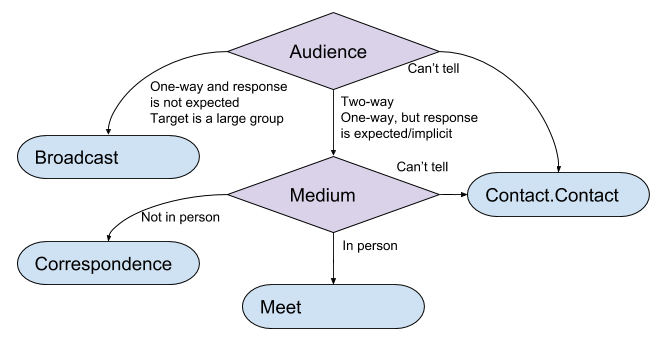
\includegraphics[width=\textwidth]{img/contact_decision_tree.png}
\caption{Contact type decision tree.}
\label{fig:contact_decision_tree}
\end{figure}

\type{Contact} events possess two attributes that are not annotated: Audience and Medium. Determining the value of these attributes will help you categorize \type{Contact} events into the correct subtype by following the decision tree given in figure \ref{fig:contact_decision_tree}.

The \textbf{Audience} attribute is Two-way if there is a back-and-forth in the contact (as with a normal conversation, phone call, interview, etc.). The Audience attribute is One-way if the communication is not or cannot be answered, or if the target (audience) of the message is a large, indefinite group of people. If it impossible to know from context, it is Can't-tell. 

Note that if the nature of the contact implies that a back-and-forth is possible or expected, even though the text only refers to one-way contact, the Audience attribute is also Two-way. This can be difficult to determine. Remember that determining the contact as One-way means the event's subtype becomes \type{Contact.Broadcast}. In some cases (like a Twitter message or a political speech) this is intuitively the right choice. In others there is more room for uncertainty. That is why we use an added criterium: a \type{Broadcast} event requires the audience to be a large group. This is not a hard constraint, but a good rule of thumb. When in doubt, it is best to note the Audience as Can't-tell, in which case the event type becomes the generic \type{Contact.Contact}.

\begin{exe}
    
    \ex \annxpl{De voormalige president maakte tijdens het \anntrg{gesprek} duidelijk dat hij zou meewerken.} 
        \expl A conversation clearly indicates two-way contact. However, we cannot determine if it happened in person or not.
        \type{Contact.Contact}.
        
    \ex \annxpl{The IMF \anntrg{report} gave some hope to countries battered by the depression.} 
        \expl A report indicates One-way contact: no reply is expected. 
        \type{Contact.Broadcast.}
        
    \ex \annxpl{Opmerkelijk is dat Zuckerberg zich liet verassen door een \anntrg{vraag} over zijn persoonlijke gegevens.} 
        \expl The sentence only mentions the one-way contact of a question being asked (there is no indication of a reply). However, it is clear from context that Zuckerberg answered or was expected to answer. The Audience is therefore Two-way. The medium is uncertain. 
        \type{Contact.Contact.}
        
    \ex \annxpl{Jan \anntrg{noemt} Bert een leugenaar.} 
        \expl Only one-way communication is attested. However, \annxpl{Bert} is not a large group of people. It is also not possible to clearly say whether a response is expected here, so we say that Audience is Can't-tell. 
        \type{Contact.Contact}
        
    \ex \annxpl{President Trump once again baffled his followers with an inflammatory \anntrg{tweet.}} 
        \expl A tweet can lead to a back-and-forth conversation through Twitter, but the sentence does not mention this. Because the tweet is sent out to a large group (Trump's twitter followers) and nothing indicates a conversation taking place, the Audience attribute is One-way. 
        \type{Contact.Broadcast.}
    
\end{exe}

The \textbf{Medium} attribute is either In-person, Not-in-person or Can't-tell. A meeting around a table happens in person; a phone call does not. It might be unclear from the sentence which it is. In this case, annotate the event as \type{Contact.Contact}. When In-person and Not-in-person contact happens in the same sentence with different verbs, it is generally advised to annotate two separate events.

\begin{exe}

    \ex \annxpl{De twee hielden nog lang \anntrg{contact} via brief en e-mail.} 
    \expl Their conversation clearly does not happen in person: \type{Contact.Correspondence.}
    
    \ex \annxpl{Naast hun \anntrg{briefwisseling} \anntrg{spraken} ze urenlang over het leven tijdens lange avondwandelingen.} 
    \expl \annxpl{Briefwisseling} denotes a Not-in-person contact event (\type{Contact.Correspondence}), while \annxpl{spraken} occurs In-person (\type{Contact.Meet}).
    
    \ex \annxpl{In \anntrg{brieven} en \anntrg{ontmoetingen} leerden ze elkaar kennen.}
    \expl Ditto: two triggers for two events, even though both events coordinate around the same fact.
    
    \ex \annxpl{Regelmatig \anntrg{contact} bracht hen samen.} 
    \expl In this case it is not possible to know whether the contact happens in person, not in person or both: \type{Contact.Contact.}
    
\end{exe}

More examples:

\begin{exe}
    
    \ex \annxpl{De aanslag van Sayfullo Saipov was een \anntrg{boodschap} voor de wereld.}
    \expl Giving a message is an act of communication. This is a clear instance of one-way communication to a large, undefined group (\annxpl{de wereld}). This leads us to \type{Contact.Broadcast}.
    
    \ex \annxpl{Alle partijen zaten gisteren rond de ronde tafel om de tarieven te \anntrg{bespreken}.} 
    \expl There is necessarily two-way communication going on between the involved parties. Since they are talking in person, this is an instance of \type{Contact.Meet}.
    
    \ex \annxpl{De president \anntrg{contacteerde} de Japanse minister om zich te verontschuldigen.} 
    \expl \annxpl{Contacteerde} implies the communication did not take place face-to-face. We can also reasonably assume that there was some back-and-forth communication: \type{Contact.Correspondence}.
    
    \ex \annxpl{Hammas issued an inflammatory \anntrg{statement}.} 
    \expl Issuing a statement, making a declaration or a speech, etc., all imply one-way communication to a large group: \type{Contact.Broadcast}.
    
    \ex \annxpl{In a groundbreaking \anntrg{report}, the UN made clear its position on climate change.}
    \expl \annxpl{Report}, rather than \annxpl{made clear}, is the trigger of a \type{Contact.Broadcast} event.
    
\end{exe}


\subsection{\type{Contact} argument roles}

\begin{figure}[t]
\centering
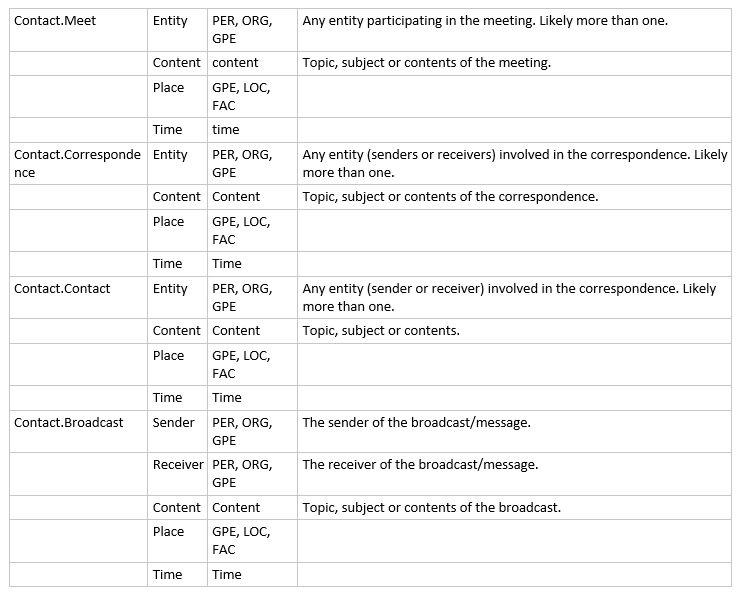
\includegraphics[width=\textwidth]{img/contact_type_args.png}
\caption{Contact type argument roles.}
\label{fig:contact_type_args.png}
\end{figure}

Allowed \type{Contact} type arguments are given in figure \ref{fig:contact_type_args.png}. The Content argument represents the content or topic of the message being transmitted. It will often be an entire relative clause, in which case you should not tag the relative pronoun.

\begin{exe}
    
    \ex \annxpl{De 33-jarige Zuckerberg \anntrg{gaf te kennen} dat \textbf{Facebook tienduizenden apps zou screenen.}} 
        \expl \type{Con\-tact.\-Broad\-cast.} The Content argument is bolded.
    
    \ex \annxpl{Alle partijen zaten gisteren rond de ronde tafel om \textbf{de tarieven} te \anntrg{bespreken.}}
        
    \ex \annxpl{Zuckerberg liet zich verassen door een \anntrg{vraag} over \textbf{zijn persoonlijke gegevens.}}

\end{exe}






\section{Dealing with quotations}

We annotate inside a quotation the same way we annotate outside of it. We do not consider the quotation to be a separate sentence. That means it is possible to identify an event outside a quotation and annotate arguments for that event inside of it, and vice-versa.

\begin{exe}
    \ex \annxpl{\emph{De politie} liet hem weten dat \emph{hij} "snel \anntrg{gearresteerd} zou worden".}
        \expl \type{Justice.ArrestJail}
        \expl Agent = De politie
        \expl Person = hij
        \expl The Person argument lies outside the quote.
\end{exe}

When the quote is the Content argument of a \type{Contact} event, it's important to remember that the inside of the message is separate from the outside of it. We take care not to associate elements inside the message with the same \type{Contact} event.

\begin{exe}
    \ex \annxpl{De \anntrg{boodschap} van de generaal was duidelijk: "IS zal nog harder \anntrg{getroffen} worden."} 
        \expl \annxpl{Boodschap} introduces a \type{Contact.\-Broad\-cast} event to which \annxpl{IS zal nog harder getroffen worden} is the Content argument. However, \annxpl{IS} is not an argument in this event. The message contains a \type{Conflict.Attack} event to which \annxpl{IS} is an argument.
\end{exe}

Sometimes, a quotation is used as the title of an article -- the quotation spans the entire sentence. In this case, no trigger can be identified, and nothing must be annotated.

\begin{exe}
    \ex \annxpl{``Spijtig dat er niet meer doden vielen.''} 
        \expl No trigger can be identified and no event is annotated.
    
    \ex \annxpl{``Spijtig dat er niet meer doden vielen,'' \anntrg{bekende} de dader achteraf.} 
        \expl The trigger is clear. The quote then serves as the Content argument to the \type{Contact.Contact} event.
\end{exe}





\chapter{Event Arguments}
\label{chapter/arguments}
TODO: \\
- CLOSEDOWN: think about Embedded Modifier Referent rule
- CLOSEDOWN: finish discussing entity types
- Find an example of p29. NOTE: one argument mention can only fill one slot: participant and filler type clash "attack on Europe" Target participant and PLACE filler. Does this happen for our types?\\
- Insert an example of scope (but use color per event type) as on p. 31.\\

This chapter describes the annotation of arguments of events.

\section*{Basic concepts and terminology}
\begin{description}[noitemsep]
    \item[Event mention] An instance of an event in full-text annotation.
    \item[Argument mention] An instance of an argument in full-text annotation.
    \item[Event mention scope] The textual scope from which arguments and attributes are tagged for a specific event mention.
    The event mention scope definition specifies the start and end of a specific event mention in the document 
    \item[Filler argument] \tagged{full}{This is the Rich ERE equivalent of "Argument Filler".}
    \item[Participant argument] \tagged{full}{This is the Rich ERE equivalent of "Event Participan Argument".}
    \item[Extent] The textual boundaries (start and end) of a linguistic expression associated with an Participant or Filler argument.
    The string of text we annotate to indicate a concept.
    The extent rules described in these guidelines define restrictions on linguistic constructions (e.g. Noun Phrase, Prepositional Phrase, Pronoun, Proper Noun, Noun, etc.) that are allowed for that category.
    Extent is different for Participant and Filler argument.
    \item[Event Role]
    \item[Taggability] The rules and circumstances in which a running full-text mention is tagged.
\end{description}

\section*{Typographical conventions}
We lay out some typographical signifiers for consistency and ease of reading:
\\[10pt]
In \textbf{text examples}: \underline{Underline} shows the event arguments or potential event argument candidates.
\textbf{Bold} indicates the event trigger.
\\[10pt]
\textbf{Event tables} take the following form:\\[10pt]
\begin{tabular}{|l|l|} \hline
\type{Type.Subtype} of event & "event trigger token span" \\\hline
\type{EventParticipantArgument} in CamelCase & "Participant argument token span" \\
\type{FILLERARGUMENT} in ALLCAPS & "Filler argument token span" \\\hline \end{tabular}
\\\\
A one sentence example containing two events:
\begin{exe}
\ex \annexe{The \underline{FDA} \anntrg{approved} \underline{the medicine} submitted by \underline{Johnson\&Johnson} in \underline{2013} and \underline{it} was \anntrg{launched} in \underline{February 2016}.}
    \expl \begin{tabular}{|L{6cm}|L{7cm}|} \hline
        \type{ProductService.Approval} & "approved" \\\hline
        \type{Approver} & "FDA" \\
        \type{Owner} & "Johnson\&Johnson" \\
        \type{ProductService} & "the medicine" \\
        \type{TIME} & "2013" \\
        \hline \end{tabular}
        \\\\ "approved" triggers \type{ProductService.Approval} event with \type{Owner} Participant argument "company", \type{ProductService} Participant argument "product line", \type{Approver} Participant argument "FDA".
    \expl \begin{tabular}{|L{6cm}|L{7cm}|} \hline
        % \rowcolor{lightergray}
        \type{ProductService.Launch} & "launched" \\\hline
        \type{Owner} & "Johnson\&Johnson" \\
        \type{ProductService} & "it" \\
        \type{TIME} & "February 2016" \\\hline \end{tabular}
        \\\\ "launched" triggers event \type{ProductService.Launch} with \type{Owner} Participant argument "company", \type{ProductService} Participant argument "it", \type{TIME} Filler argument "2016".
\end{exe}

\section{Conceptually: arguments in events.}
Events describe changing state in the world and encapsulate actions, relations, occurrences, etc.
These involve multiple participating entities who are involved in one way or other:
as agents (causers/initiators), patients (targets/undergoers, themes), qualifiers, quantifiers, specifiers and other descriptive modifiers.
Examples are the person or company doing the action, the amount of shares involved or some other piece of information, like the place where the event happens.
%Arguments together with the event trigger form the most basic description of an event instance.

Each event has a number of corresponding arguments.
We label arguments for each event mention.
For each event, \textbf{arguments fill a number of roles specific to the event type.}
The \type{Conflict.Attack} event type, for instance, asks for an Attacker, a Target, an Instrument, a Place and a Time.\\

INSERT EXAMPLE\\

We distinguish between two types of arguments:
\begin{enumerate}
    \item \textbf{Participant} arguments: these are the text spans describing a participant that is involved in the event. 
    For each type/subtype of event there will be a specific set of participant roles to be filled. \fullref{chapter/eventtype} describes what these slots are in detail.
    \item \textbf{Filler} arguments:
    Filler arguments are not central participants in the event but provide descriptive and discriminative information.
    They denote the the time, place, title, age, crime, commodity attached to an event.
    They serve as extra but vital information in characterizing the event.
    Filler arguments differ from Participant in two ways:
    i) they are not bound by event scope mention and can be tagged anywhere in the document.
    ii) They have to be full Noun Phrases (NP), unlike Participants that can be anaphoric pronouns.
    For Filler arguments, the closest full NP mention will be tagged instead.
\end{enumerate}

\section{Technically: taggability of arguments.}
Here we explain the general technical rules for tagging event arguments that \textbf{apply to both Participant and Filler arguments}.
Most important are trigger proximity and the possible absence of arguments.\\

\noindent\textbf{Argument slots can be left empty} if the relevant argument is not mentioned in the sentence.
It is possible that some events have no explicit arguments in the sentence: their entire argument list is empty.
We expect event triggers with empty arguments to be a rare, but occur in two contexts: 
\begin{enumerate}
    \item As a violation of Event mention scope:
        \begin{exe}
        \ex \annexe{\exargpart{Disney} \anntrg{premiered} its new movie Frozen. The \anntrg{release} received universal praise.}
            \expl \begin{tabular}{|L{6cm}|L{7cm}|} \hline
                \type{ProductService.Launch} & "release" \\\hline
                \type{Owner} & \\
                \type{ProductService} & \\
                \hline \end{tabular}
            \expl "release" triggers an \type{ProductService.Launch}, conceptually the \type{Owner}
        \end{exe}
\end{enumerate}

\noindent\textbf{Shared argument rule}:
When a candidate argument mention is also an argument in a different, non-coreferent event it is annotated.
Events can be co-related and similar, but not coreferent:
Non-coreferent events do not have the same \type{Type.Subtype} or do not refer to same exact event instance.
For Participant argument, this does not violate the event mention scope boundary and Participants can be tagged.

In these examples, the over- and underlined $\overline{\underline{argument}}$ should attach to both different event mentions in \anntrg{bold}:
\begin{samepage}
\begin{exe}
\ex \annexe{The \underline{FDA} \anntrg{approved} \underline{the medicine} submitted by $\overline{\underline{Johnson\&Johnson}}$ in \underline{2013} and \underline{it} was \anntrg{launched} in \underline{February 2016}.}
    \nopagebreak
        \expl \begin{tabular}{|L{6cm}|L{7cm}|} \hline
            \type{ProductService.Approval} & "approved" \\\hline
            \type{Approver} & "FDA" \\
            $\overline{\underline{\type{Owner}}}$ & "Johnson\&Johnson" \\
            \type{ProductService} & "the medicine" \\
            \type{TIME} & "2013" \\
            \hline \end{tabular}
        \expl \begin{tabular}{|L{6cm}|L{7cm}|} \hline
            % \rowcolor{lightergray}
            \type{ProductService.Launch} & "launched" \\\hline
            $\overline{\underline{\type{Owner}}}$ & "Johnson\&Johnson" \\
            \type{ProductService} & "it" \\
            \type{TIME} & "February 2016" \\\hline \end{tabular}
        \expl This is an instance of shared Participant arguments.
    \ex  \annexe{Amazon opened a new \anntrg{distribution center} in \underline{Glendale} where they secured a \anntrg{tax abatement deal} with local government.}
        \expl "distribution center" \type{Facility.Open} event with \type{Owner} Participant argument "Amazon", \type{Facility} Participant argument "distribution center", \type{Place} Filler argument "Glendale".
        \expl "tax abatement deal" \type{Deal} with \type{Partner} Participant argument "they", \type{Partner} Participant argument "local government", shared \type{Place} Filler argument "Glendale".
        \expl This is an instance of shared Filler arguments.
\end{exe}
\end{samepage}

\noindent
\textbf{Trigger Proximity Rule}:
In complex sentences, a single argument to an event can be mentioned more than once. 
In that case, we annotate the mention that is \textbf{closest to the trigger}.\\

\noindent\textbf{Saliency Rule}:
When one argument mention has multiple plausible role candidates for the same event:
Exceptionally, an argument mention corresponds to two role slots of the same event.
In this case, choose the most salient role.
The most salient role is the one that is most important to interpreting the event and distinguishing it from other event types or subtypes.

\begin{exe}
    \ex \annexe{The \underline{company} \anntrg{approved} the product line.}
        \expl "approved" \type{ProductService.Approval} with two plausible candidates as Participant arguments for "company" as specified in the event typology: \type{Owner} and \type{Approver}. The company is both the approving entity for the product and owner of the product.
        \expl \type{Approver} is the correct Participant argument tag as it characterizes the event better.
\end{exe}

\noindent\textbf{Embedded Modifier Referent rule}:
We allow overlapping annotations in cases where a modifier of an argument itself refers to a taggable argument.

\begin{exe}
    \ex The \exargfill{law-firm} is \anntrg{litigating a class action lawsuit} against \exargpart{Ford Motor Company} for [\exargfill{the recall of defective [Takata] airbags}]. In turn, \exargpart{Ford} is \anntrg{seeking damages} for \exargfill{the faulty parts}.
    \expl \begin{tabular}{|L{6cm}|L{7cm}|} \hline
        \type{Legal.Proceeding} & "litigating a class action lawsuit" \\\hline
        \type{Defendant} & "Ford" \\
        \type{Complainant} & "law-firm" \\
        \type{Adjudicator} &  \\
        \type{ALLEGATION} & "the recall of defective Takata airbags" \\
        \hline \end{tabular}
    \expl \begin{tabular}{|L{6cm}|L{7cm}|} \hline
        \type{Legal.Proceeding} & "seeking damages" \\\hline
        \type{Defendant} & "Takata" \\
        \type{Complainant} & "Ford" \\
        \type{Adjudicator} &  \\
        \type{ALLEGATION} & "the faulty parts" \\
        \hline \end{tabular}
    \expl these are two distinct events in which [Takata] serves as the \type{Defendant} Participant argument of the second event while being a modifier of the first event argument filler. 
\end{exe}

\textbf{Coordinated arguments rule}:
Multiple events can be started by one trigger when arguments are coordinated and they are clearly distinct events.
However, argument coordination can also indicate one event with multiple arguments filling the same role.
These rules help you decide whether to tag one event with multiple arguments in the same role or two events:
\begin{enumerate}
    \item If the TIME and PLACE Filler arguments are different or there are separate times and places indicated for coordinated arguments, tag two separate events.
    \item If any other Participant or Filler argument is coordinated, tag a single event.
    In this case there will be multiple arguments filling the same event argument role.
    \item If distinguishing between one or multiple events is too complicated, default to annotating a single event with multiple arguments.
\end{enumerate}

\begin{exe}
    \ex The motor manufacturer plans to launch a sedan and a hatchback in Korea.
        \expl \begin{tabular}{|L{6cm}|L{7cm}|} \hline
            % \rowcolor{lightergray}
            \type{ProductService.Launch} & "launch" \\\hline
            $\overline{\underline{\type{Owner}}}$ & "Johnson\&Johnson" \\
            \type{ProductService} & "a sedan" \\
            \type{ProductService} & "a hatchback" \\
            \type{PLACE} & "Korea" \\\hline \end{tabular}
    \expl One event triggered by "launch" of type \type{Product.Launch} with two ProductService participant arguments, one for "a sedan" and one for "a hatchback".
    \ex The motor manufacturer plans to launch a sedan in China and a hatchback in Korea.
        \expl \begin{tabular}{|L{6cm}|L{7cm}|} \hline
            \type{ProductService.Launch} & "launch" \\\hline
            $\overline{\underline{\type{Owner}}}$ & "Johnson\&Johnson" \\
            \type{ProductService} & "a sedan" \\
            \type{PLACE} & "China" \\\hline \end{tabular}
        \expl \begin{tabular}{|L{6cm}|L{7cm}|} \hline
            \type{ProductService.Launch} & "launch" \\\hline
            $\overline{\underline{\type{Owner}}}$ & "Johnson\&Johnson" \\
            \type{ProductService} & "a hatchback" \\
            \type{PLACE} & "Korea" \\\hline \end{tabular}
        \expl Two separate events triggered by "launch" of type \type{Product.Launch} with one ProductSevice argument each.
    \ex The stock fell to 11USD yesterday and today to 10.78USD.
        \expl Two separate events for trigger "fell" of type \type{SecurityPrice}.
\end{exe}

\textbf{General note on argument Extent}:
Your task is to find each taggable argument mention in the document, and label its extent – that is, the string of text that refers to the argument as a potentially discontinuous span of tokens.
Mention extents generally begin and end at word (token) boundaries.

However, possessive endings ('s) and verbal contractions (‘m, ‘ve, ‘re) should be excluded from the mention extent.
These are treated as if they were separate tokens and are already tokenized in the annotation interface.
As a rule, you should also exclude punctuation characters like commas, periods, and quotation marks unless the same entity mention continues after the punctuation mark.

\section{Participant Taggability}

We distinguish two types of arguments: Participant and Filler arguments.
This section discusses the annotation rules for Participant arguments.
Their taggability is mainly different from Fillers by the Event Mention Scope and their extent.

A Participant argument is any entity that participates in a \tagged{full}{taggable} event mention.
An entity is a unique object or set of objects in the world.
For instance, a specific company, person, place, product or organization that is involved in the action of the event. 
A Participant argument mention is a single occurrence of a \textbf{name}, \textbf{noun phrase}, or \textbf{pronominal phrase} that refers to, or describes, a single participant role.
These specific participant roles are listed in \fullref{chapter/eventtype}.
% The mention extent is a string of text that we annotate to indicate the occurrence of an argument mention. We link together multiple mentions of the same argument during entity coreference annotation.

\textbf{Event mention scope rule}:
We \textbf{only tag Participant argument mentions that occur within the event mention scope} for an event trigger.
The event mention scope is defined as the span of a document from the first trigger of an event to the next trigger you see for the same, coreferent event.
Event mention scopes do not begin and end at the trigger words themselves, but at sentence boundaries:
\textbf{The scope of an event spans to the start of the trigger sentence to the start if the sentence of the next \underline{coreferent} event.}
Note that this means not any next event but the next coreferent event, i.e. with the same type.subtype referring to the same conceptual event.
(Event coreference is described in \fullref{chapter/coref}.)
Non-coreferent events do not end the event mention scope.

Always tag arguments closest to the event trigger.

INSERT EXAMPLE FIGURE AS IN PAGE 31 of Rich ERE Event Guidelines.

This rule does not apply to Argument Fillers.
Unlike Participant arguments, Filler arguments are not bound by event mention scope and can be tagged anywhere in the document.
Always tag the closest Filler argument mention to the event trigger as per Proximity Rule.

\noindent\textbf{We only annotate arguments to a taggable event.}
We annotate events first, then look for the participant role (or Filler argument) that the event requires. 
If an entity does not have a role as an event argument, we do not annotate it.\\

\subsection{Participant extent rules}
Here we discuss the rules for selecting which tokens are allowed in annotation of a Participant argument.
Special rules for argument extents apply depending on whether they are nominal or pronominal mentions.\\

\noindent\textbf{Nominal} Participant arguments:
Nominal Participant argument mentions are realized by a noun or full noun phrase with constituents (NP).
This means we tag the full NP with children for nominally realized Participants.
Appositive and relative clauses are included as long as they are children/dependent of the argument NP.
This has the potential for long token span arguments, but we expect overly complex NPs to be rare.
Proper names, acronyms, nicknames, aliases, abbreviations, ticker symbols, or another alternate names are nominal participant arguments.
Names will be tagged since they constitute NPs on their own or are part of NPs and are not given special treatment.

In the following examples, the correct participant extent is [\exargpart{underlined and bracketed}].
\begin{itemize}[noitemsep]
    \item {\exargpart{[XYZ , another large company whose investors revolted]} underwent similar troubles.}
    \item {\exargpart{Bill Robertson , the youngest XYZ Corp. executive}}, will
    \item {[\exargpart{Apple 's former CEO Steve Jobs}]} ' replacement was announced today.
    \item {[The \exargpart{Denver Broncos} sports team] entered into a sponsorship deal with [\exargpart{XYZ Corp}].}
    \item {[\exargpart{The company 's baseline}] will likely benefit from [\exargfill{president Trump 's tax reform}]}
    \item {[\exargpart{Microsoft}]} aka [\exargpart{MS}] aka [\exargpart{MSFT}] (ticker)
    \item {[\exargpart{Pharma giant Johnson \& Johnson}]} announced breakthrough results [...]
    \item {[\exargpart{Bill}]} and [\exargpart{Melinda Gates}]: see coordinated arguments.
    \item {[\exargpart{The company which earlier proclaimed the merits of this feature}]} now admits to the scandal.
\end{itemize}

\noindent\textbf{Pronominal participant arguments}:
A pronominal argument mention is a referring expression that corresponds to a nominal or named entity.
\textbf{The extent of a pronominal mention is just the single referring unit, typically a pronoun.}

Below is a list of English pronouns/pronominal mentions. 
Note that NPs starting with any of these words are not pronouns but NPs (e.g., "this bank", "the other board members", "few of the products" are nominal NP mentions).
Pronominal usage is a requisite.

\begin{multicols}{5}
\setlength\multicolsep{0pt}
\begin{itemize}[noitemsep]
    \item all \item another \item any \item both \item each 
    \item each other \item either \item everybody \item everyone \item everything \item few
    \item he \item her \item hers \item herself \item him 
    \item himself \item his \item I \item it \item its 
    \item itself \item little \item many \item me \item mine
    \item more \item most \item much \item my \item myself 
    \item one \item one another \item other \item others \item our 
    \item ours \item ourselves \item several \item she \item some 
    \item somebody \item someone \item something \item that \item their 
    \item theirs \item them \item themselves \item these \item they 
    \item this \item those \item us \item we \item what 
    \item whatever \item where \item wherever \item which \item whichever 
    \item who \item whoever \item whom \item whomever \item whose 
    \item you \item your \item yours \item yourself
\end{itemize}
\end{multicols}

\noindent\textbf{Reflexive pronouns} are arguments the same as other pronouns.
However the pronominal argument can fill a seperate role from its nominal referent in some special cases:

\begin{exe}
    \ex \exargpart{The CEO} was pressured into \anntrg{firing} \exargpart{himself}.
        \expl "fire" triggers \type{Employment.End} event with "The CEO" in the \type{Employer} and "himself" in the \type{employee} role.
\end{exe}

\noindent\textbf{Relative pronouns} are tagged when they are the closest Participant argument mention to the event.
This happens when the event trigger is part of a relative clause.

\begin{exe}
    \ex The manufacturer, \exargpart{which} \anntrg{laid off} \exargpart{200 factory line workers} in \exargfill{2016}, is now facing declining sales.
        \expl "laid off" triggers \type{Employment.End} event with "which" in the \type{Employer} role.
\end{exe}


\section{Canonical coreferent for pronominal mentions}
When a pronominal participant argument is tagged, we annotate a coreference link to the most canonical mention of that entity in the document.
This does not necessarily mean that we annotate a coreferent link to the nearest nominal coreferent mention.
We link to the mention that best identifies and uniquely characterizes the referent of the pronominal mention.
The goal is to obtain a highly referential mention for that entity that uniquely identifies the pronominal argument mention in question.

The most canonical referent likely includes a proper name or is a definite, highly referential NP if a proper name is lacking in the document.

In the following example the canonical coreferent is shown in [ square brackets ].
\begin{exe}
    \ex {[ Alphabet Inc. ]} unveiled new information about their secretive "moonshot" research center "X". This fits in a recent trend of openness taken by the holding. The technology conglomerate which recently announced \exargpart{it} is testing a drone delivery service has been more willing to lift the veil on ongoing projects.
        \expl Alphabet Inc. is the most canonical mention for referent "it". Other coreferent mentions are "the holding", "The technology conglomerate", and "which", but "Alphabet Inc." is chosen because it is the most unique identifier of that referent.
\end{exe}

Preference is given to proper names.
If the proper name is part of an NP, tagging only the proper name suffices: there is no need to tag the full NP.
When there are multiple plausible candidates, choose the coreferent nominal mention closest to the event trigger in the document.

This coreference link is annotated primarily to disambiguate the argument and not for full coreference resolution purposes.

\tagged{full}{
\subsection{Differences with Rich ERE entity extent}
Named entities in Rich ERE are tagged as distinct of nominal entities.
Even though proper names are constituent parts of a full NP they are tagged separately.
We do not make this distinction as a simplification as we do not need the same entity level granularity as ERE.
This removes the need for specifying rules for headless NPs, named+nominal combinations, and partitive constructions (e.g. "all of the board", "one of the companies").

Unlike Rich ERE, we also do not tag the head of the NP as a simplification. When needed in processing, we leave determining the head of the NP to syntactic dependency parsers.
For relative clauses a distinction between specifying and non-specifying clauses would be useful, but we do not provide such annotations.
}
 
\section{Filler Argument Taggability}
The Filler argument extent is the string of text we annotate to indicate a Filler argument.
The rules for identifying the extent of a Filler argument will vary from type to type.
This information is given for each specific Filler type in \fullref{chapter/events}.

Many Filler arguments are mentioned by a noun phrase (NP).
The extent of a Filler argument is the entire NP unless otherwise specified for its type.
When it is difficult to decide if modifiers should be included or not, the Filler argument extent should be maximally inclusive.
In the case of a discontinuous extent, the extent goes to the end of the constituent, even if that means including tokens that are not part of the constituent.
For example:
\begin{exe}
    \ex The law-firm litigates \anntrg{a class action lawsuit} against \exargfill{Ford} for \exargfill{the bodged recall in 2018 of the} \exargfill{defective Takata airbags}.
    \expl The extent of the ALLEGATION Filler argument [the bodged recall in 2018 of the defective Takata airbags]\textsubscript{ALLEGATION} contains pre-modifiers "the bodged" and prepositional phrase "in 2018" and runs until "airbags". The mention of "the recall" being due to "defective Takata airbags" is essential to the description of the event.
\end{exe}

The extent includes all the modifiers of an NP, including determiners, prepositional phrases, appositive phrases and relative clauses.

Unlike Participant arguments, we do not annotate pronominal mentions for Fillers (e.g. "where" for PLACE and "when" for TIME) and tag the nominal mention closest to the event trigger.


\section{Realis of arguments}
The link between each event argument and its event trigger will be labeled with a realis attribute.
Realis of arguments is independent from the event trigger and its other arguments.
The realis attribute of an argument will only apply to the relationship of that particular argument to the event.

The default value is ACTUAL, which is not marked. Only IRREALIS is marked when the argument is not asserted as a participant or filler in the event mention.



\chapter{Event Coreference}
\label{chapter/coref}
The final annotation step is that of linking coreferent events in the document.
This means you annotate a link between event triggers that intuitively refer to the same real-world event.\\[10pt]
\noindent
The criteria for linking coreferent event mentions:
\begin{enumerate}[noitemsep]
    \item \textbf{Semantically and intuitively} refer to the same real-world event.
    \item \textbf{\type{Type} and \type{Subtype} are identical}.
    \item \textbf{Temporal and location scope are identical}, but the time and place expressions do not have to be exactly the same (e.g., \annexe{"The product launch in 2017"} and \annexe{"Last year's product release"}, \annexe{"The company opens its new headquarters in Detroit"} and \annexe{"the real-estate investment in Motor City"} use different expressions to denote the same point in time or space).
    The place and time do not have to be exactly the same but \textbf{correspond in scope} (e.g., \annexe{"six month ago"} and \annexe{"last year"} are in the same temporal scope, \annexe{"Canada and the US" and "North-America"} are in the same location scope).
    Time periods/points and locations are coreferent as long as the roughly fit into each other.
    \item Not necessarily the same arguments:
    Argument mentions do not have to be identical.
    However, the referred arguments will roughly correspond in their referents.
    Arguments can be left implied, specified, or generalized but do not have to be exactly identical.
    \item Not necessarily the same trigger.
    \item Not necessarily the same Factuality.
\end{enumerate}

\noindent
Note that \textbf{events with same \type{Type.Subtype} and corresponding place/time are not automatically coreferent}:
Annotators should always infer from context and meaning that they are indeed the same real-world event involving the same entities, persons, companies, etc.
For example: \annexe{"XYZ Corp. ended their cloud computing service in 2017. [...] Last year they stopped their service contract with ABC Inc."} have the same \type{Product.CancellationRecall} type and subtype and are within the same temporal scope, but refer to distinct events by way of having clearly separate involved arguments.\\

\noindent
Many events will not have coreferent events in the document.

\tagged{full}{
\section{Correspondence to Event Hoppers in Rich ERE}
For event coreference, we directly inherited Rich ERE's concept of event hoppers. \cite{LDC2016.rich_ere}
A hopper is a group of annotated events that refer to the same event occurrence.
This differs from strict event coreference in ACE and Light ERE in which arguments also have to corefer strictly.

Quoting \cite{LDC2016.rich_ere}:

\begin{quote}
    Tagged event mentions that refer to the same event occurrence will be grouped into Event Hoppers. 
    Event Hopper is a more inclusive, less strict notion of event coreference as compared to strict event coreference in ACE and Light ERE. Event hoppers contain mentions of events that “feel” coreferential to the annotator even if they do not meet the earlier strict event identity requirement. More specifically, event mentions that have the following features go into the same hopper:
\end{quote}

Rich ERE event hopper criteria can be summarized as follows:
\begin{itemize}[noitemsep]
    \item They have the same event type and subtype.
    \item They have the same temporal and location scope, though not necessarily the same temporal expression or specifically the same date (Attack in Baghdad on Thursday vs. Bombing in the Green Zone last week).
    \item Trigger granularity can be different (assaulting 32 people vs. wielded a knife).
    \item Event arguments may be non-coreferential or conflicting (18 killed vs. dozens killed).
    \item Realis status may be different (will travel [OTHER] to Europe next week vs. is on a 5-day trip [ACTUAL])
\end{itemize}
}


\chapter{Event Typology}
\label{chapter/eventtype}
\renewcommand*{\arraystretch}{1.3}
\newcommand*{\thline}{\specialrule{.1em}{.05em}{.05em}}
\renewcommand*\thesubsection{\arabic{subsection}}

\titleformat*{\section}{\justify\LARGE\bfseries}
\titleformat*{\subsection}{\justify\Large\bfseries}

\let\oldminipage=\minipage
\let\endoldminipage=\endminipage
\renewenvironment{minipage}{\vspace{-2.5mm}\begin{oldminipage}}{\end{oldminipage}\vspace{2mm}}

\setcounter{section}{-1}

\section{Typographical convention}

\centering\begin{tabularx}{\textwidth}{| L{2.55cm} L{6cm} L{6.3cm} |}
\multicolumn{3}{C{14.85cm}}{\Large \textbf{EventType\_Subtype}}                \\
\specialrule{.1em}{.05em}{.05em} 
\multicolumn{2}{|L{8.55cm}}{
	\begin{minipage}{8.55cm}
		A description of the event type or subtype.
	\end{minipage}
	} & \annexe{Event mention example sentence with the trigger word in \anntrg{bold}.} \\ \thline
ParticipantArgument & Description of the Participant argument. & \annexe{Participant argument example sentence with the argument \exargpart{highlighted}} \\
FILLERARGUMENT & Brief description of FILLER argument. For full description for FILLER arguments see \ref{sec:FILLERtypes}. Note: TIME and PLACE FILLERs are allowed on all event types and are not included in event type overviews. & \annexe{FILLER argument example sentence with the FILLER argument \exargfill{highlighted}.}  \\
\specialrule{.1em}{.05em}{.05em} 
\end{tabularx}

\section{Event types}

%-------CSR/Brand----------
\subsection{CSR/Brand}

\centering\begin{tabularx}{\textwidth}{| L{2.55cm} L{6cm} L{6.3cm} |}
\multicolumn{3}{C{14.85cm}}{\Large \textbf{CSR/Brand}}                \\
\specialrule{.1em}{.05em}{.05em} 
\multicolumn{2}{|L{8.55cm}}{
	\begin{minipage}{8.55cm}
		Corporate Social Responsibility and Branding events take place when the company's effects on environmental and social wellbeing are assessed or when the brand image is affected. Includes environmental and social efforts (e.g. affirmative action, employee well-being) and scandals violating responsibility such as sexism accusations, corruption, bribing, etc. Branding includes events improving or damaging image and credibility of the brand image, company image, or product image. This includes advertising campaigns, affiliations, sponsorships.
	\end{minipage}
	} & \annexe{example}                                                                         \\ \thline
Company & The company or brand directly associated with the CSR/Brand event  & \annexe{Argument 1 example sentence with the argument highlighted} \\
\specialrule{.1em}{.05em}{.05em} 
\end{tabularx}

\begin{itemize}[noitemsep,leftmargin=*]
	\item Keywords: Scandal, Corruption, Social Responsibility, Environmental Responsibility, Company Image, Brand Image, Product Image, Credibility, Award, Sponsorship, Advertising Campaign, Affiliation.
	\item \url{en.wikipedia.org/wiki/Corporate_social_responsibility}
	\item \url{www.investopedia.com/terms/c/corp-social-responsibility.asp}
\end{itemize}

\vspace{0.5cm}

%-------Capital Returns----------
\subsection{Capital Returns}
\centering\begin{tabularx}{\textwidth}{| L{2.55cm} L{6cm} L{6.3cm} |}
\multicolumn{3}{C{14.85cm}}{\Large \textbf{CapitalReturns}}                \\
\specialrule{.1em}{.05em}{.05em} 
\multicolumn{2}{|L{8.55cm}}{
	\begin{minipage}{8.55cm}
		A company returns capital to its shareholders. The typical methods are Stock Buy Backs (or Share Repurchases) and Dividends.
	\end{minipage}
	} & \annexe{example}                                                                         \\ \thline
Returnee & The company giving out dividends or buying back its stock  & \annexe{Argument 1 example sentence with the argument highlighted} \\
Amount & Amount of capital returned to the company in monetary amount, amount of shares bought-back, or dividends payed-out.  & \annexe{Argument 2 example sentence with the argument highlighted}  \\
\specialrule{.1em}{.05em}{.05em}
\end{tabularx}

\begin{itemize}[noitemsep,leftmargin=*]
	\item \url{www.investopedia.com/terms/r/returnofcapital.asp}
	\item \url{www.investopedia.com/terms/b/buyback.asp}
	\item \url{en.wikipedia.org/wiki/Share_repurchase}
	\item \url{corporatefinanceinstitute.com/resources/knowledge/finance/dividend-vs-share-buyback-repurchase/}
	\item \url{https://en.wikipedia.org/wiki/Dividend}
	\item \url{https://www.investopedia.com/terms/d/dividendyield.asp}
\end{itemize}

\vspace{0.5cm}

\centering\begin{tabularx}{\textwidth}{| L{2.55cm} L{6cm} L{6.3cm} |}
\multicolumn{3}{C{14.85cm}}{\Large CapitalReturns\_\textbf{ShareRepurchase}}                \\
\specialrule{.1em}{.05em}{.05em} 
\multicolumn{2}{|L{8.55cm}}{
	\begin{minipage}{8.55cm}
		Share repurchase (or stock buyback) is the re-acquisition by a company of its own stock.
		A share repurchase is a program by which a company buys back its own shares from the marketplace, usually because management thinks the shares are undervalued, and thereby reducing the number of outstanding shares. 
		The company buys shares directly from the market or offers its shareholders the option of tendering their shares directly to the company at a fixed price.
	\end{minipage}
	} & \annexe{example}                                                                         \\ \thline
Returnee & The company giving out dividends or buying back its stock  & \annexe{Argument 1 example sentence with the argument highlighted} \\
Amount & Amount of capital returned to the company in monetary amount, amount of shares bought-back, or dividends payed-out.  & \annexe{Argument 2 example sentence with the argument highlighted}  \\
Price & Unit price of the shares. & \\
\specialrule{.1em}{.05em}{.05em}
\end{tabularx}

\vspace{0.5cm}

\centering\begin{tabularx}{\textwidth}{| L{2.55cm} L{6cm} L{6.3cm} |}
\multicolumn{3}{C{14.85cm}}{\Large CapitalReturns\_\textbf{DividendPayment}}                \\
\specialrule{.1em}{.05em}{.05em} 
\multicolumn{2}{|L{8.55cm}}{
	\begin{minipage}{8.55cm}
		A dividend is a payment made by a corporation to its shareholders, usually as a distribution of profits.
		When a corporation earns a profit or surplus, the corporation is able to re-invest the profit in the business (called retained earnings) and pay a proportion of the profit as a dividend to shareholders.
		Distribution to shareholders may be in cash (usually a deposit into a bank account).
	\end{minipage}
	} & \annexe{example}                                                                         \\ \thline
Returnee & The company giving out dividends or buying back its stock  & \annexe{Argument 1 example sentence with the argument highlighted} \\
Amount & Amount of capital returned to the company in monetary amount, amount of shares bought-back, or dividends payed-out.  & \annexe{Argument 2 example sentence with the argument highlighted}  \\
YieldRatio & The current dividend yield ratio in percentage. &                                    \\
\specialrule{.1em}{.05em}{.05em} 
\end{tabularx}

\vspace{0.5cm}

\centering\begin{tabularx}{\textwidth}{| L{2.55cm} L{6cm} L{6.3cm} |}
\multicolumn{3}{C{14.85cm}}{\Large CapitalReturns\_\textbf{DividendYieldRaise}}                \\
\specialrule{.1em}{.05em}{.05em} 
\multicolumn{2}{|L{8.55cm}}{
	\begin{minipage}{8.55cm}
		The dividend yield ratio has increased over a period and has changed substantially as a positive percentage increase compared to a historical trend.
		The dividend yield is a financial ratio that indicates how much a company pays out in dividends each year relative to its share price.
		Dividend yield is represented as a percentage and can be calculated by dividing the dollar value of dividends paid in a given year per share of stock held by the dollar value of one share of stock.
	\end{minipage}
	} & \annexe{example}                                                                         \\ \thline
Returnee & The company giving out dividends or buying back its stock  & \annexe{Argument 1 example sentence with the argument highlighted} \\
Amount & Capital returned to the company in gross monetary amount, amount of shares bought-back, or dividends payed-out.  & \annexe{Argument 2 example sentence with the argument highlighted}  \\
YieldRatio & The current dividend yield ratio in percentage. &                                    \\
HistoricalYieldRatio & The dividend yield ratio in percentage compared to which the current yield ratio has increased. &        \\
\specialrule{.1em}{.05em}{.05em} 
\end{tabularx}

\vspace{0.5cm}

\centering\begin{tabularx}{\textwidth}{| L{2.55cm} L{6cm} L{6.3cm} |}
\multicolumn{3}{C{14.85cm}}{\Large CapitalReturns\_\textbf{DividendYieldReduction}}                \\
\specialrule{.1em}{.05em}{.05em} 
\multicolumn{2}{|L{8.55cm}}{
	\begin{minipage}{8.55cm}
		The dividend yield ratio has decreased over a period and has changed substantially as a negative percentage decrease compared to a historical trend.
		The dividend yield is a financial ratio that indicates how much a company pays out in dividends each year relative to its share price.
		Dividend yield is represented as a percentage and can be calculated by dividing the dollar value of dividends paid in a given year per share of stock held by the dollar value of one share of stock.
	\end{minipage}
	} & \annexe{example}                                                                         \\ \thline
Returnee & The company giving out dividends or buying back its stock  & \annexe{Argument 1 example sentence with the argument highlighted} \\
Amount & Capital returned to the company in monetary amount, amount of shares bought-back, or dividends payed-out.  & \annexe{Argument 2 example sentence with the argument highlighted}  \\
YieldRatio & The current dividend yield ratio in percentage. &                                    \\
HistoricalYieldRatio & The dividend yield ratio in percentage compared to which the current yield ratio has decreased. &        \\
 & & \\
\specialrule{.1em}{.05em}{.05em} 
\end{tabularx}

\vspace{0.5cm}

\centering\begin{tabularx}{\textwidth}{| L{2.55cm} L{6cm} L{6.3cm} |}
\multicolumn{3}{C{14.85cm}}{\Large CapitalReturns\_\textbf{DividendYieldStable}}                \\
\specialrule{.1em}{.05em}{.05em} 
\multicolumn{2}{|L{8.55cm}}{
	\begin{minipage}{8.55cm}
		The dividend yield ratio has remained stable over a period and has not changed substantially compared to a historical trend.
		The dividend yield is a financial ratio that indicates how much a company pays out in dividends each year relative to its share price.
		Dividend yield is represented as a percentage and can be calculated by dividing the dollar value of dividends paid in a given year per share of stock held by the dollar value of one share of stock. 
	\end{minipage}
	} & \annexe{example}                                                                         \\ \thline
Returnee & The company giving out dividends or buying back its stock  & \annexe{Argument 1 example sentence with the argument highlighted} \\
Amount & Capital returned to the company in monetary amount, amount of shares bought-back, or dividends payed-out.  & \annexe{Argument 2 example sentence with the argument highlighted}  \\
YieldRatio & The current dividend yield ratio in percentage. &                                    \\
HistoricalYieldRatio & The dividend yield ratio in percentage compared to which the current yield ratio has remained stable. &        \\
\specialrule{.1em}{.05em}{.05em} 
\end{tabularx}

\vspace{0.5cm}

%-------Deal---------
\subsection{Deal}

\centering\begin{tabularx}{\textwidth}{| L{2.55cm} L{6cm} L{6.3cm} |}
\multicolumn{3}{C{14.85cm}}{\Large \textbf{Deal}}                \\
\specialrule{.1em}{.05em}{.05em} 
\multicolumn{2}{|L{8.55cm}}{
	\begin{minipage}{8.55cm}
		Deals and partnerships to cooperate with another company or entity. Service and product deals, licensing, contract bid, alliance, partnership, Memorandum of Understanding (MOU), pacts, joint ventures (two companies pool resources to accomplish a task), collaborations, contracts, agreements, development partnerships (usually public private partnerships for development projects), and affiliations.
	\end{minipage}
	} & \annexe{example}                                                                         \\ \thline
Partner & One of the partner in the deal. A deal by definition has multiple partners. & \annexe{Argument 1 example sentence with the argument highlighted} \\
Goal & Goal and aims of the deal. & \\

\specialrule{.1em}{.05em}{.05em} 
\end{tabularx}
Keywords: Service and product deals, licensing, contract bid, alliance, partnership, Memorandum of Understanding (MOU), pacts, joint ventures (two companies pool resources to accomplish a task), collaborations, contracts, agreements, development partnerships (usually public private partnerships for development projects), and affiliations.
\begin{itemize}
	\item \url{en.wikipedia.org/wiki/Corporate_social_responsibility}
\end{itemize}

\vspace{0.5cm}

%-------Employment---------
\subsection{Employment}

\centering\begin{tabularx}{\textwidth}{| L{2.55cm} L{6cm} L{6.3cm} |}
\multicolumn{3}{C{14.85cm}}{\Large \textbf{Employment}}                \\
\specialrule{.1em}{.05em}{.05em} 
\multicolumn{2}{|L{8.55cm}}{
	\begin{minipage}{8.55cm}
		Events regarding employment changes (firing and hiring), compensation, and issues regarding the workforce or other employees such as executives.
		Includes CEO changes, executive change, board change, executive compensation, employment issues, strikes, workforce increase, workforce decrease/firing.
	\end{minipage}
	} & \annexe{example}                                                                         \\ \thline
Employee & Employee, group of employees, part of the workforce. & \annexe{Argument 2 example sentence with the argument highlighted}  \\
Employer & Employer company or employing person.  & \annexe{Argument example sentence with the argument highlighted} \\
TITLE & The job title/position of the employee. & \annexe{FILLER example sentence with the argument highlighted} \\
\specialrule{.1em}{.05em}{.05em} 
\end{tabularx}

\vspace{0.5cm}

\centering\begin{tabularx}{\textwidth}{| L{2.55cm} L{6cm} L{6.3cm} |}
\multicolumn{3}{C{14.85cm}}{\Large Employment\_\textbf{Start}}                \\
\specialrule{.1em}{.05em}{.05em}
\multicolumn{2}{|L{8.55cm}}{
	\begin{minipage}{8.55cm}
		A person or group of people start a new job position at an employer (company or organization). Includes events, announcements, speculation, expectation, changes on hiring, CEO changes, executive change, board change, workforce increases.
	\end{minipage}
	} & \annexe{example}                                                                         \\ \thline
Employee & Employee, group of employees, part of the workforce starting a new position. & \annexe{Argument 2 example sentence with the argument highlighted}  \\
Employer & Employer company or employing person.  & \annexe{Argument example sentence with the argument highlighted} \\
Replacing & The person that the starting Employee replaces. & \annexe{Argument example sentence with the argument highlighted}\\
TITLE & The job title/position of the starting Employee. & \annexe{Argument example sentence with the argument highlighted} \\
\specialrule{.1em}{.05em}{.05em} 
\end{tabularx}

\vspace{0.5cm}

\centering\begin{tabularx}{\textwidth}{| L{2.55cm} L{6cm} L{6.3cm} |}
\multicolumn{3}{C{14.85cm}}{\Large Employment\_\textbf{End}}                \\
\specialrule{.1em}{.05em}{.05em} 
\multicolumn{2}{|L{8.55cm}}{
	\begin{minipage}{8.55cm}
		The job position of a person or a group of people has ended with an employer (company or organization). Includes events, announcements, speculation, expectation, changes CEO change, executive change, board change, workforce decrease/firing, termination, death, illness, and any other form of ending a professional position.
	\end{minipage}
	} & \annexe{example}                                                                         \\ \thline
Employee & Employee, group of employees, part of the workforce being terminated/fired. & \annexe{Argument 2 example sentence with the argument highlighted}  \\
Employer & Employer company or employing person doing the firing.  & \annexe{Argument example sentence with the argument highlighted} \\
Replacer & The person that replaces the terminated Employee. & \annexe{Argument example sentence with the argument highlighted}\\
TITLE & The job title/position of the terminated Employee. & \annexe{Argument example sentence with the argument highlighted} \\

\specialrule{.1em}{.05em}{.05em} 
\end{tabularx}

\vspace{0.5cm}

\centering\begin{tabularx}{\textwidth}{| L{2.55cm} L{6cm} L{6.3cm} |}
\multicolumn{3}{C{14.85cm}}{\Large Employment\_\textbf{Compensation}}                \\
\specialrule{.1em}{.05em}{.05em} 
\multicolumn{2}{|L{8.55cm}}{
	\begin{minipage}{8.55cm}
		Changes in compensation for employees. Executive compensation as equity, workforce pay-out, payment issues, or wage in/decreases.
	\end{minipage}
	} & \annexe{example}                                                                         \\ \thline
Employee & Employee, group of employees, part of the workforce who's compensation is affected. & \annexe{Argument 2 example sentence with the argument highlighted}  \\
Employer & Employer company or employing person.  & \annexe{Argument example sentence with the argument highlighted} \\
Amount & the monetary amount of compensation. & \\
TITLE & The job title/position of the terminated Employee. & \annexe{Argument example sentence with the argument highlighted} \\
\specialrule{.1em}{.05em}{.05em} 
\end{tabularx}

\vspace{0.5cm}

\centering\begin{tabularx}{\textwidth}{| L{2.55cm} L{6cm} L{6.3cm} |}
\multicolumn{3}{C{14.85cm}}{\Large Employment\_\textbf{Problem}}                \\
\specialrule{.1em}{.05em}{.05em} 
\multicolumn{2}{|L{8.55cm}}{
	\begin{minipage}{8.55cm}
		Issues, strikes, hiring failure, and other problems regarding employment.
	\end{minipage}
	} & \annexe{example}                                                                         \\ \thline
Employee & Employee, group of employees, part of the workforce who is involved in a problem. & \annexe{Argument 2 example sentence with the argument highlighted}  \\
Employer & Employer company or employing person.  & \annexe{Argument example sentence with the argument highlighted} \\
TITLE & The job title/position of the terminated Employee. & \annexe{Argument example sentence with the argument highlighted} \\
\specialrule{.1em}{.05em}{.05em} 
\end{tabularx}
Note: has overlap with CSR/Brand.

\vspace{0.5cm}

%-------Facility---------
\subsection{Facility}

\centering\begin{tabularx}{\textwidth}{| L{2.55cm} L{6cm} L{6.3cm} |}
\multicolumn{3}{C{14.85cm}}{\Large \textbf{Facility}}                \\
\specialrule{.1em}{.05em}{.05em} 
\multicolumn{2}{|L{8.55cm}}{
	\begin{minipage}{8.55cm}
		Events pertaining to a company's physical presence as facilities, factories, headquarters, warehouses, and other real-estate. Facilities opening, facilities closing, headquarters relocation, headquarters opening, headquarters closing. Facilities include headquarters, retail sites, production sites, logic centers, etc.
	\end{minipage}
	} & \annexe{example}                                                                         \\ \thline
Facility & Facility, factory or headquarters. & \annexe{Argument 2 example sentence with the argument highlighted}  \\
Company & Company that is owner of the facility or headquarters.  & \annexe{Argument 1 example sentence with the argument highlighted} \\

\specialrule{.1em}{.05em}{.05em} 
\end{tabularx}

\vspace{0.5cm}

\centering\begin{tabularx}{\textwidth}{| L{2.55cm} L{6cm} L{6.3cm} |}
\multicolumn{3}{C{14.85cm}}{\Large Facility\_\textbf{Open}}                \\
\specialrule{.1em}{.05em}{.05em} 
\multicolumn{2}{|L{8.55cm}}{
	\begin{minipage}{8.55cm}
		Facilities opening, includes headquarters, factories, production sites, retail sites, etc.
	\end{minipage}
	} & \annexe{example}                                                                         \\ \thline
Facility & Facility or headquarters & \annexe{Argument 2 example sentence with the argument highlighted}  \\
Company & Company opening facility or headquarters.  & \annexe{Argument 1 example sentence with the argument highlighted} \\

\specialrule{.1em}{.05em}{.05em} 
\end{tabularx}

\vspace{0.5cm}

\centering\begin{tabularx}{\textwidth}{| L{2.55cm} L{6cm} L{6.3cm} |}
\multicolumn{3}{C{14.85cm}}{\Large Facility\_\textbf{Close}}                \\
\specialrule{.1em}{.05em}{.05em} 
\multicolumn{2}{|L{8.55cm}}{
	\begin{minipage}{8.55cm}
		Facilities closing, includes headquarters, factories, production sites, retail sites, etc.
	\end{minipage}
	} & \annexe{example}                                                                         \\ \thline
Facility & Facility or headquarters & \annexe{Argument 2 example sentence with the argument highlighted}  \\
Company & Company opening facility or headquarters.  & \annexe{Argument 1 example sentence with the argument highlighted} \\
\specialrule{.1em}{.05em}{.05em} 
\end{tabularx}

\vspace{0.5cm}

%-------FinancialResult---------
\subsection{Financial Result}

\centering\begin{tabularx}{\textwidth}{| L{2.55cm} L{6cm} L{6.3cm} |}
\multicolumn{3}{C{14.85cm}}{\Large \textbf{FinancialResult}}                \\
\specialrule{.1em}{.05em}{.05em} 
\multicolumn{2}{|L{8.55cm}}{
	\begin{minipage}{8.55cm}
		Financial results as discussed in reports published by the company or other instance.
		Quarterly and annual reports include key accounting and financial data for a company, including gross revenue, net profit, operational expenses and cash flow.
		A quarterly report for a public company typically includes an income statement, balance sheet, and cash flow statement for the quarter and the year-to-date (YTD), as well as comparative results for the prior year.
		This event captures publishing, announcement or discussions of these reports and reported results within them.\\
		Overlap with \type{Financing}, \type{Investment}, \type{Profit/Loss}, \type{Revenue}, \type{Sales Volume}: \type{FinancialResult}
		Result contained in these reports should be tagged into these more specific event types.
		\type{FinancialResult} is more general than these types and should be tagged when talking about a report or when the result does not fit in the more specific categories.
	\end{minipage}
	} & \annexe{example}                                                                         \\ \thline
Reportee & Company that is the topic of the financial report. & \\
Result & The type of result with associated monetary amount that is reported on. & \\
\specialrule{.1em}{.05em}{.05em} 
\end{tabularx}

\vspace{0.5cm}

\centering\begin{tabularx}{\textwidth}{| L{2.55cm} L{6cm} L{6.3cm} |}

\multicolumn{3}{C{14.85cm}}{\Large FinancialResult\_\textbf{Beat}}                \\
\specialrule{.1em}{.05em}{.05em} 
\multicolumn{2}{|L{8.55cm}}{
	\begin{minipage}{8.55cm}
		A financial report shows that a company's financials are better than previous expectations or historical trends.
	\end{minipage}
	} & \annexe{example}                                                                         \\ \thline
Reportee & Company that is the topic of the financial report. & \\
Result & The type of result with associated monetary amount that is reported on. & \\
\specialrule{.1em}{.05em}{.05em} 
\end{tabularx}

\vspace{0.5cm}

\centering\begin{tabularx}{\textwidth}{| L{2.55cm} L{6cm} L{6.3cm} |}

\multicolumn{3}{C{14.85cm}}{\Large FinancialResult\_\textbf{Miss}}                \\
\specialrule{.1em}{.05em}{.05em} 
\multicolumn{2}{|L{8.55cm}}{
	\begin{minipage}{8.55cm}
		A financial report shows that a company's financials are worse than previous expectations or historical trends.
	\end{minipage}
	} & \annexe{example}                                                                         \\ \thline
Reportee & Company that is the topic of the financial report. & \\
Result & The type of result with associated monetary amount that is reported on. & \\
\specialrule{.1em}{.05em}{.05em} 
\end{tabularx}

\vspace{0.5cm}

\centering\begin{tabularx}{\textwidth}{| L{2.55cm} L{6cm} L{6.3cm} |}

\multicolumn{3}{C{14.85cm}}{\Large FinancialResult\_\textbf{Stable}}                \\
\specialrule{.1em}{.05em}{.05em} 
\multicolumn{2}{|L{8.55cm}}{
	\begin{minipage}{8.55cm}
		A financial report shows that a company's financials are stable or as expected w.r.t. previous expectations or historical trends.
	\end{minipage}
	} & \annexe{example}                                                                         \\ \thline
Reportee & Company that is the topic of the financial report. & \\
Result & The type of result with associated monetary amount that is reported on. & \\
\specialrule{.1em}{.05em}{.05em} 
\end{tabularx}

\vspace{0.5cm}

%-------Financing---------
\subsection{Financing}

\centering\begin{tabularx}{\textwidth}{| L{2.55cm} L{6cm} L{6.3cm} |}
\multicolumn{3}{C{14.85cm}}{\Large \textbf{Financing}}                \\
\specialrule{.1em}{.05em}{.05em} 
\multicolumn{2}{|L{8.55cm}}{
	\begin{minipage}{8.55cm}
		Financing of a company are ways in which it raises capital through debt and equity.
		Equity financing involves not just the sale of stocks, but also the sale of other equity or quasi-equity instruments such as preferred stock, convertible preferred stock and equity units that include common shares and warrants.
		These events focus on how a company raises equity through issuing shares in IPOs, stock splits, etc.
		Debt Financing refers to the way in which companies raise funds by taking on debt by issuing bonds or taking on loans. Debt financing occurs when a firm sells fixed income products, such as bonds, bills, or notes, to investors.
		Event mentions pertaining to company debt and debt ratios. Includes debt announcements, debt forecasts, debt increases, debt reductions, and debt and equity restructuring.
		The balance between equity and debt of a company is expressed as the weighted average cost of capital, or WACC.
		\\
		Overlap with \type{Ratings\_Debt} and \type{Investment}.
		Difference with \type{Ratings\_Debt} that this is not a rating by an analyst. \type{Financing} events are focused around a company taking on debt to raise capital.
		Difference with \type{Investment} is that \type{Financing} events are focused around means of raising capital and not the investor-investee relation in se.
	\end{minipage}
	} & \annexe{example}                                                                         \\ \thline
Financee & The company selling equity as shares or taking on debt by issuing bonds or taking out loans. & \\
Financer & The company, institution, or private entity investing in equity or giving out the loan. & \\
Amount & Amount of capital financed as debt or equity. & \\
\specialrule{.1em}{.05em}{.05em} 
\end{tabularx}

\begin{itemize}[noitemsep,leftmargin=*]
    \item \url{https://www.investopedia.com/terms/d/debtfinancing.asp}
    \item \url{https://www.investopedia.com/terms/e/equityfinancing.asp}
    \item \url{https://www.investopedia.com/ask/answers/032515/how-does-company-choose-between-debt-and-equity-its-capital-structure.asp}
    \item \url{https://www.investopedia.com/financial-edge/1112/small-business-financing-debt-or-equity.aspx}
    \item \url{https://finance.zacks.com/differences-between-debt-equity-investments-3035.html}
    \item \url{https://corporatefinanceinstitute.com/resources/knowledge/finance/debt-vs-equity/}
    \item \url{https://www.investopedia.com/terms/b/bond.asp}
\end{itemize}

\vspace{0.5cm}

%-------Investment---------
\subsection{Investment}

\centering\begin{tabularx}{\textwidth}{| L{2.55cm} L{6cm} L{6.3cm} |}
\multicolumn{3}{C{14.85cm}}{\Large \textbf{Investment}}                \\
\specialrule{.1em}{.05em}{.05em} 
\multicolumn{2}{|L{8.55cm}}{
	\begin{minipage}{8.55cm}
		Investment in other companies or subsidiaries.
		This event involves one company investing in another company it owns as a subsidiary or does not control or own fully as in affiliate/associate companies.
		Corporate investments are often Capital Investments as part of a Corporate Finance strategy.
		This event has overlap with i) MergerAcquisition and ii) Deal: i) the difference between MergerAcquisition and Investment is that in the MergerAcquisition event one company gains full ownership of another company or parts of that company. This is not the case in Investment where partial ownership through share investment is possible but not the goal. ii) Deal is more general than Investment, an Investment is between two companies with the investing party investing some capital expecting a return. A Deal can be between any two entities and is much more general regarding its meaning.
	\end{minipage}
	} & \annexe{example}                                                                         \\ \thline
Investor & Company or organization that makes the investment. & \\
Investee & Company being in which the Investor invests. Can also be a stock or other security. & \\
CapitalInvested & Amount of capital invested as a monetary expression. & \\
\specialrule{.1em}{.05em}{.05em} 
\end{tabularx}

\begin{itemize}[noitemsep,leftmargin=*]
	\item \url{https://www.investopedia.com/terms/c/capital-investment.asp}
	\item cf. Capital Investment \url{https://www.investopedia.com/terms/c/corporatefinance.asp}
\end{itemize}

\vspace{0.5cm}

%-------Legal---------
\subsection{Legal}

\centering\begin{tabularx}{\textwidth}{| L{2.55cm} L{6cm} L{6.3cm} |}
\multicolumn{3}{C{14.85cm}}{\Large \textbf{Legal}}                \\
\specialrule{.1em}{.05em}{.05em} 
\multicolumn{2}{|L{8.55cm}}{
	\begin{minipage}{8.55cm}
		Events pertaining to governmental justice. Investigations. accusations, litigations, arrest charges, Fraud, Money Laundering, Bribing, Settlement, Judgement, Lawsuit, Legal issues, Regulatory issues, injunctions.
	\end{minipage}
	} & \annexe{example}
\\ \thline
Defendant & Entity, company, or person being alleged of a crime, under investigation, convicted, fined, etc. & \\
ALLEGATION & Allegation or other formal/legal offence that is alleged against a Defendant. & \\
\specialrule{.1em}{.05em}{.05em} 
\end{tabularx}

\vspace{0.5cm}

\centering\begin{tabularx}{\textwidth}{| L{2.55cm} L{6cm} L{6.3cm} |}
\multicolumn{3}{C{14.85cm}}{\Large Legal\_\textbf{Proceeding}}                \\
\specialrule{.1em}{.05em}{.05em} 
\multicolumn{2}{|L{8.55cm}}{
	\begin{minipage}{8.55cm}
		A court proceeding has been initiated for a defendant accused of an allegation. Legal proceedings include trials, lawsuits, and hearings. Trials are state-initiated proceedings in a court. Hearing are state-initiated proceedings outside the court (e.g. in Senate). Lawsuits are proceedings between private parties. This also includes charges and indictments, i.e. formal accusations, and investigations.
	\end{minipage}
	} & \annexe{example}                                                                         \\ \thline
Defendant & Entity being convicted, fined, etc. & \\
Complainant & Entity filing suit or initiating the proceeding by accusation of the defendant. Governmental prosecutor, plaintiff, litigator, suer, petitioner. & \\
Adjudicator & Judge or court. In case of investigation, the investigator either private by attorney or public police investigators. & \\
ALLEGATION & Allegation or other formal/legal offence that is alleged against a Defendant. & \\
\specialrule{.1em}{.05em}{.05em} 
\end{tabularx}

\vspace{0.5cm}

\centering\begin{tabularx}{\textwidth}{| L{2.55cm} L{6cm} L{6.3cm} |}
\multicolumn{3}{C{14.85cm}}{\Large Legal\_\textbf{Conviction/Settlement}}                \\
\specialrule{.1em}{.05em}{.05em} 
\multicolumn{2}{|L{8.55cm}}{
	\begin{minipage}{8.55cm}
		A defendant has been found guilty of an allegation and is at the conclusion of a trial.
		The defendant is convicted to a sentence which can be jail-time, a fine, cease-and-desist, etc.
		Also applies where allegations are settled out of court.
	\end{minipage}
	} & \annexe{example}                                                                         \\ \thline
Defendant & Entity being convicted, fined, etc. & \\
Adjudicator & Entity proclaiming the conviction & \\
SENTENCE & Sentence, fine, incarceration, or other punishment. & \\
ALLEGATION & Allegation or other formal/legal offence that is alleged against a Defendant. & \\

\specialrule{.1em}{.05em}{.05em} 
\end{tabularx}

\vspace{0.5cm}

\centering\begin{tabularx}{\textwidth}{| L{2.55cm} L{6cm} L{6.3cm} |}
\multicolumn{3}{C{14.85cm}}{\Large Legal\_\textbf{Acquit}}                \\
\specialrule{.1em}{.05em}{.05em} 
\multicolumn{2}{|L{8.55cm}}{
	\begin{minipage}{8.55cm}
		A defendant has been found not guilty of an allegation at the conclusion of a trial. This is the opposite of conviction.
	\end{minipage}
	} & \annexe{example}                                                                         \\ \thline
Defendant & Entity being convicted, fined, etc. & \\
Adjudicator & Entity proclaiming the conviction. & \\
ALLEGATION & Allegation or other formal/legal offence that is alleged against a Defendant. & \\
\specialrule{.1em}{.05em}{.05em}
\end{tabularx}

\vspace{0.5cm}

\centering\begin{tabularx}{\textwidth}{| L{2.55cm} L{6cm} L{6.3cm} |}
\multicolumn{3}{C{14.85cm}}{\Large Legal\_\textbf{Appeal}}                \\
\specialrule{.1em}{.05em}{.05em} 
\multicolumn{2}{|L{8.55cm}}{
	\begin{minipage}{8.55cm}
		A court decision is taken to a higher court for review.
	\end{minipage}
	} & \annexe{example}                                                                         \\ \thline
Defendant & Entity being convicted, fined, etc. & \\
Complainant & Entity filing suit or initiating the proceeding by accusation of the defendant. Governmental prosecutor, plaintiff, litigator, sue-er, petitioner. & \\
Adjudicator & Entity proclaiming the conviction. & \\
ALLEGATION & Allegation or other formal/legal offence that is alleged against a Defendant. & \\
\specialrule{.1em}{.05em}{.05em} 
\end{tabularx}

\vspace{0.5cm}

%-------Macroeconomics---------
\subsection{Macroeconomics}

\centering\begin{tabularx}{\textwidth}{| L{2.55cm} L{6cm} L{6.3cm} |}
\multicolumn{3}{C{14.85cm}}{\Large \textbf{Macroeconomics}}                \\
\specialrule{.1em}{.05em}{.05em} 
\multicolumn{2}{|L{8.55cm}}{
	\begin{minipage}{8.55cm}
		Macro-economic events are aggregated indicators such as sectorial trends, policy, GDP, unemployment rates, national income, price indices, and the interrelations among the different markets and sectors of the economy. Includes events, speculation, expectation, forecasts, announcements, changes on a company's position in the marker, the state of the market, sector or country in general,  headwinds, tailwinds, business trends, market share, consumer spending, etc.
	\end{minipage}
	} & \annexe{example}                                                                         \\ \thline
AffectedCompany & Company, organization, or entity being affected by the macroeconomic event. & \\
Sector & Sector, industry, market, state, geographical location where the event takes effect. & \\
\specialrule{.1em}{.05em}{.05em} 
\end{tabularx}

\vspace{0.5cm}


%-------Merger/Acquisition---------
\subsection{Merger/Acquisition}

\centering\begin{tabularx}{\textwidth}{| L{2.55cm} L{6cm} L{6.3cm} |}
\multicolumn{3}{C{14.85cm}}{\Large \textbf{Merger/Acquisition}}                \\
\specialrule{.1em}{.05em}{.05em} 
\multicolumn{2}{|L{8.55cm}}{
	\begin{minipage}{8.55cm}
		Consolidation of companies and assets involving at least two companies. A merger is a legal consolidation of two entities into one entity. An acquisition occurs when one entity takes ownership of another entity's stock, equity interests or assets.
	\end{minipage}
	} & \annexe{example}                                                                         \\ \thline
Acquirer & Entity receiving the company or assets & \\
Target & Entity filing suit or initiating the proceeding by accusation of the defendant. Governmental prosecutor, plaintiff, litigator, suer, petitioner. & \\
Cost & Cost of the merger or acquisition in monetary amount. & \\
\specialrule{.1em}{.05em}{.05em} 
\end{tabularx}

\vspace{0.5cm}


%-------Product/Service---------
\subsection{Product/Service}

\centering\begin{tabularx}{\textwidth}{| L{2.55cm} L{6cm} L{6.3cm} |}
\multicolumn{3}{C{14.85cm}}{\Large \textbf{Product/Service}}                \\
\specialrule{.1em}{.05em}{.05em} 
\multicolumn{2}{|L{8.55cm}}{
	\begin{minipage}{8.55cm}
		Events pertaining to a product or service. Includes announcements, launches, testing, changes, up/downgrades, updates, recalls, trial results, approvals, reviews, and other issues regarding products and services of a company.
	\end{minipage}
	} & \annexe{example}                                                                         \\ \thline
ProductService & The Product/Service in question. & \\
Producer & Company, organization, or entity that produces, delivers, or otherwise brings to market the product or service. & \\
\specialrule{.1em}{.05em}{.05em} 
\end{tabularx}

\vspace{0.5cm}

\centering\begin{tabularx}{\textwidth}{| L{2.55cm} L{6cm} L{6.3cm} |}
\multicolumn{3}{C{14.85cm}}{\Large Product/Service\_\textbf{Launch}}                \\
\specialrule{.1em}{.05em}{.05em} 
\multicolumn{2}{|L{8.55cm}}{
	\begin{minipage}{8.55cm}
		A company brings a new product/service to market. Also applicable to product and service updates.
	\end{minipage}
	} & \annexe{example}                                                                         \\ \thline
ProductService & Product/Service being launched. & \\
Producer & Company, organization, or entity that launches (or updates) a new product or service. & \\
\specialrule{.1em}{.05em}{.05em} 
\end{tabularx}

\vspace{0.5cm}

\centering\begin{tabularx}{\textwidth}{| L{2.55cm} L{6cm} L{6.3cm} |}
\multicolumn{3}{C{14.85cm}}{\Large Product/Service\_\textbf{Cancellation/Recall}}                \\
\specialrule{.1em}{.05em}{.05em} 
\multicolumn{2}{|L{8.55cm}}{
	\begin{minipage}{8.55cm}
		A company recalls a product or cancels a product/service.
	\end{minipage}
	} & \annexe{example}                                                                         \\ \thline
ProductService & Product/service being launched & \\
Producer & Company, organization, or entity that recalls or cancels a product or service. & \\
\specialrule{.1em}{.05em}{.05em} 
\end{tabularx}

\vspace{0.5cm}

\centering\begin{tabularx}{\textwidth}{| L{2.55cm} L{6cm} L{6.3cm} |}
\multicolumn{3}{C{14.85cm}}{\Large Product/Service\_\textbf{Trial}}                \\
\specialrule{.1em}{.05em}{.05em} 
\multicolumn{2}{|L{8.55cm}}{
	\begin{minipage}{8.55cm}
		A product or service is being tested or trialed either by a company or regulatory body.\\
		This includes testing runs of prototypes, and approval or disapproval after trial by regulatory agents or governments.
		This type is typical for reporting on bio-technology and pharmaceutical industries which require trial by a regulatory body. Technology and consumers products/services are also often trialed before being brought to market.
	\end{minipage}
	} & \annexe{example} \\ \thline
ProductService & Product/service being launched & \\
Producer & Company, organization, or entity that is testing the product/service. & \\
Trialer & Governmental or private regulator, organization, or other entity overseeing the trial. & \\                    
\specialrule{.1em}{.05em}{.05em}
\end{tabularx}

\vspace{0.5cm}

%-------Profit/Loss---------
\subsection{Profit/Loss}

\centering\begin{tabularx}{\textwidth}{| L{2.55cm} L{6cm} L{6.3cm} |}
\multicolumn{3}{C{14.85cm}}{\Large \textbf{Profit/Loss}}                \\
\specialrule{.1em}{.05em}{.05em} 
\multicolumn{2}{|L{8.55cm}}{
	\begin{minipage}{8.55cm}
		Profits are financial benefits that are realized when the amount of revenue exceeds expenses. Inversely, losses happen when the expense exceeds the revenue. We include declarations and forecasts of profit/loss, positive and negative (losses) profit, lower than, higher than, as expected, increased, decreased, and stable profits. Has conceptual overlap with Revenue.
	\end{minipage}
	} & \annexe{example} \\ \thline
Profiteer & Company, organization, or entity turning a profit or loss. & \\
Amount & The amount of money won/lost. & \\
\specialrule{.1em}{.05em}{.05em} 
\end{tabularx}

\vspace{0.5cm}

\centering\begin{tabularx}{\textwidth}{| L{2.55cm} L{6cm} L{6.3cm} |}
\multicolumn{3}{C{14.85cm}}{\Large Profit/Loss\_\textbf{Increase}}                \\
\specialrule{.1em}{.05em}{.05em} 
\multicolumn{2}{|L{8.55cm}}{
	\begin{minipage}{8.55cm}
        Profit or Loss has increased compared to a historical trend. We do not differentiate between Profit and Loss: this event applies to whichever is the topic of topic of the event.\\
		Overlap with \type{Revenue}:
	\end{minipage}
	} & \annexe{example}    \\ \thline
Profiteer & Company, organization, or entity turning a profit or loss. & \\
Amount & The current amount of money won/lost. & \\
HistoricalAmount & The historical amount of money won or lost compared to which the current amount is higher. & \\
\specialrule{.1em}{.05em}{.05em} 
\end{tabularx}

\vspace{0.5cm}

\centering\begin{tabularx}{\textwidth}{| L{2.55cm} L{6cm} L{6.3cm} |}
\multicolumn{3}{C{14.85cm}}{\Large Profit/Loss\_\textbf{Decrease}}                \\
\specialrule{.1em}{.05em}{.05em} 
\multicolumn{2}{|L{8.55cm}}{
	\begin{minipage}{8.55cm}
        Profit or Loss has decreased compared to a historical trend. We do not differentiate between Profit and Loss: this event applies to whichever is the topic of topic of the event.\\
		Overlap with \type{Revenue}:
	\end{minipage}
	} & \annexe{example}       \\ \thline
Profiteer & Company, organization, or entity turning a profit or loss. & \\
Amount & The current amount of money won/lost. & \\
HistoricalAmount & The historical amount of money won or lost compared to which the current amount is lower. & \\
\specialrule{.1em}{.05em}{.05em} 
\end{tabularx}

\vspace{0.5cm}

\centering\begin{tabularx}{\textwidth}{| L{2.55cm} L{6cm} L{6.3cm} |}
\multicolumn{3}{C{14.85cm}}{\Large Profit/Loss\_\textbf{Decrease}}                \\
\specialrule{.1em}{.05em}{.05em} 
\multicolumn{2}{|L{8.55cm}}{
	\begin{minipage}{8.55cm}
        Profit or Loss has decreased compared to a historical trend. We do not differentiate between Profit and Loss: this event applies to whichever is the topic of topic of the event.\\
		Overlap with \type{Revenue}:
	\end{minipage}
	} & \annexe{example}                                                                         \\ \thline
Profiteer & Company, organization, or entity turning a profit or loss. & \\
Amount & The current amount of money won/lost. & \\
HistoricalAmount & The historical amount of money won or lost compared to which the current amount is lower. & \\
\specialrule{.1em}{.05em}{.05em} 
\end{tabularx}

\vspace{0.5cm}

\centering\begin{tabularx}{\textwidth}{| L{2.55cm} L{6cm} L{6.3cm} |}
\multicolumn{3}{C{14.85cm}}{\Large Profit/Loss\_\textbf{Stable}}                \\
\specialrule{.1em}{.05em}{.05em} 
\multicolumn{2}{|L{8.55cm}}{
	\begin{minipage}{8.55cm}
        Profit or Loss has remained stable or there is no significant change compared to a historical trend. We do not differentiate between Profit and Loss: this event applies to whichever is the topic of topic of the event.\\
		Overlap with \type{Revenue}:
	\end{minipage}
	} & \annexe{example}                                                                         \\ \thline
Profiteer & Company, organization, or entity turning a profit or loss. & \\
Amount & The current amount of money won/lost. & \\
HistoricalAmount & The historical amount of money won or lost compared to which the current amount remained stable. & \\
\specialrule{.1em}{.05em}{.05em} 
\end{tabularx}

\vspace{0.5cm}


%-------Rating---------
\subsection{Rating}

\centering\begin{tabularx}{\textwidth}{| L{2.55cm} L{6cm} L{6.3cm} |}
\multicolumn{3}{C{14.85cm}}{\Large \textbf{Rating}}                \\
\specialrule{.1em}{.05em}{.05em} 
\multicolumn{2}{|L{8.55cm}}{
	\begin{minipage}{8.55cm}
		Analyst ratings and advice on securities such as stocks but also credit and debt ratings. Includes announcements, forecasts, speculation, expectation, reports, etc. on analyst ratings, analyst advice, analysts setting Price targets, analysts credit-debt ratings, changes in rating agency listing, or buy/sell/hold and upgrade/downgrade/maintain advice.
	\end{minipage}
	} & \annexe{example}                                                                         \\ \thline
Security & Security or company's debt being rated. & \\
Analyst & Rater, advisor or analyst publishing the rating. & \\
\specialrule{.1em}{.05em}{.05em} 
\end{tabularx}

\begin{itemize}
    \item \url{https://www.investopedia.com/financial-edge/0512/understanding-analyst-ratings.aspx}
\end{itemize}

\vspace{0.5cm}

\centering\begin{tabularx}{\textwidth}{| L{2.55cm} L{6cm} L{6.3cm} |}
\multicolumn{3}{C{14.85cm}}{\Large Rating\_\textbf{BuyOutperform}}                \\
\specialrule{.1em}{.05em}{.05em} 
\multicolumn{2}{|L{8.55cm}}{
	\begin{minipage}{8.55cm}
		Analyst advises to buy a security. "Outperform" signals an analyst recommendation a stock is expected to do slightly better than the market return. Buy and outperform can also be expressed as "overweight", "moderate buy", "accumulate", "add", "buy" and "strong buy" advice.
	\end{minipage}
	} & \annexe{example}                                                                         \\ \thline
Security & Security being rated. & \\
Analyst & Rater, advisor or analyst publishing the rating. & \\
\specialrule{.1em}{.05em}{.05em} 
\end{tabularx}

\vspace{0.5cm}

\centering\begin{tabularx}{\textwidth}{| L{2.55cm} L{6cm} L{6.3cm} |}
\multicolumn{3}{C{14.85cm}}{\Large Rating\_\textbf{SellUnderperform}}                \\
\specialrule{.1em}{.05em}{.05em}
\multicolumn{2}{|L{8.55cm}}{
	\begin{minipage}{8.55cm}
		Analyst advises to sell a security or liquidate an asset. "Underperform" signals a recommendation that a stock is expected to do slightly worse than the overall stock market return. Sell or underperform can also be expressed as "moderate sell," "weak hold" and "underweight.". Includes "underweight", "underperform", "moderate sell", and "sell" and "strong sell" advice.
	\end{minipage}
	} & \annexe{example}                                                                         \\ \thline
Security & Security being rated. & \\
Analyst & Rater, advisor or analyst publishing the rating. & \\
\specialrule{.1em}{.05em}{.05em} 
\end{tabularx}

\vspace{0.5cm}

\centering\begin{tabularx}{\textwidth}{| L{2.55cm} L{6cm} L{6.3cm} |}
\multicolumn{3}{C{14.85cm}}{\Large Rating\_\textbf{Hold}}                \\
\specialrule{.1em}{.05em}{.05em} 
\multicolumn{2}{|L{8.55cm}}{
	\begin{minipage}{8.55cm}
	    Analyst advises to hold a security. A hold recommendation signals a security is expected to perform at the same pace as comparable companies or in-line with the market. Includes "hold" and "neutral" advice.
	\end{minipage}
	} & \annexe{example}                                                                         \\ \thline
Security & Security being rated. & \\
Analyst & Rater, advisor or analyst publishing the rating. & \\
\specialrule{.1em}{.05em}{.05em} 
\end{tabularx}

\vspace{0.5cm}

\centering\begin{tabularx}{\textwidth}{| L{2.55cm} L{6cm} L{6.3cm} |}

\multicolumn{3}{C{14.85cm}}{\Large Rating\_\textbf{Upgrade}}                \\
\specialrule{.1em}{.05em}{.05em} 
\multicolumn{2}{|L{8.55cm}}{
	\begin{minipage}{8.55cm}
		Analyst ratings, credit rating or advice are upgraded from an (implied) previous rating.
		For stocks, a "hold" advice can be upgrade to a "buy" advice.
		A "sell" advice can be upgraded to a "hold" or "buy" advice.
	\end{minipage}
	} & \annexe{example}                                                                         \\ \thline
Security & Security being rated. & \\
Analyst & Rater, advisor or analyst publishing the rating. & \\
HistoricalRating & The previous rating from which the security is upgraded. & \\
\specialrule{.1em}{.05em}{.05em} 
\end{tabularx}

\vspace{0.5cm}

\centering\begin{tabularx}{\textwidth}{| L{2.55cm} L{6cm} L{6.3cm} |}

\multicolumn{3}{C{14.85cm}}{\Large Rating\_\textbf{Downgrade}}                \\
\specialrule{.1em}{.05em}{.05em} 
\multicolumn{2}{|L{8.55cm}}{
	\begin{minipage}{8.55cm}
		Analyst ratings, credit rating or advice are upgraded from an (implied) previous rating.
		For stocks, a "buy" advice can be downgraded to a "hold" or a "sell" advice.
		A "hold" advice can be downgraded to a "sell" advice.
	\end{minipage}
	} & \annexe{example}                                                                         \\ \thline
Security & Security being rated. & \\
Analyst & Rater, advisor or analyst publishing out the rating. & \\
HistoricalRating & The previous rating from which the security is downgraded. & \\
\specialrule{.1em}{.05em}{.05em} 
\end{tabularx}

\vspace{0.5cm}

\centering\begin{tabularx}{\textwidth}{| L{2.55cm} L{6cm} L{6.3cm} |}

\multicolumn{3}{C{14.85cm}}{\Large Rating\_\textbf{Maintain}}                \\
\specialrule{.1em}{.05em}{.05em} 
\multicolumn{2}{|L{8.55cm}}{
	\begin{minipage}{8.55cm}
		Analyst security ratings, credit rating or advice remain in the same category from an (implied) previous rating.
	\end{minipage}
	} & \annexe{example}                                                                         \\ \thline
Security & Security being rated. & \\
Analyst & Rater, advisor or analyst publishing the rating. & \\
HistoricalRating & The previous rating from which the security remains stable. & \\
\specialrule{.1em}{.05em}{.05em} 
\end{tabularx}

\vspace{0.5cm}

\centering\begin{tabularx}{\textwidth}{| L{2.55cm} L{6cm} L{6.3cm} |}

\multicolumn{3}{C{14.85cm}}{\Large Rating\_\textbf{PriceTarget}}                \\
\specialrule{.1em}{.05em}{.05em} 
\multicolumn{2}{|L{8.55cm}}{
	\begin{minipage}{8.55cm}
		Analyst projects a price target for a security.
		A price target is the projected price level of a financial security stated by an investment analyst or advisor and includes assumptions of future activity.
		It represents a security's price that, if achieved, results in a trader recognizing the best possible outcome for his investment.
		This is the price at which the trader or investor wants to exit his existing position so he can realize the most reward.
	\end{minipage}
	} & \annexe{example}                                                                         \\ \thline
Security & Security being rated. & \\
Analyst & Rater, advisor or analyst publishing the rating. & \\
TargetPrice & The target price or value of a security as a range or singular price expressed as monetary value. & \\
\specialrule{.1em}{.05em}{.05em} 
\end{tabularx}

\vspace{0.5cm}

\centering\begin{tabularx}{\textwidth}{| L{2.55cm} L{6cm} L{6.3cm} |}

\multicolumn{3}{C{14.85cm}}{\Large Rating\_\textbf{Credit/Debt}}                \\
\specialrule{.1em}{.05em}{.05em} 
\multicolumn{2}{|L{8.55cm}}{
	\begin{minipage}{8.55cm}
		Analyst credit or debt rating for a company or organization.
		A corporate credit rating is an opinion of an independent agency regarding the likelihood that a corporation will fully meet its financial obligations as they come due.
		A company’s corporate credit rating indicates its relative ability to pay its creditors and gives investors an idea of how the company’s debt securities should be priced in term of yields.
		Credit assessment and evaluation for companies and governments is generally done by a credit rating agency such as Standard \& Poor’s (S\&P), Moody’s, or Fitch. 
	\end{minipage}
	} & \annexe{example}                                                                         \\ \thline
Security & Security being rated. & \\
Analyst & Rater, advisor or analyst publishing the rating. & \\
\specialrule{.1em}{.05em}{.05em} 
\end{tabularx}

\begin{itemize}[noitemsep,leftmargin=*]
	\item \url{https://www.investopedia.com/terms/c/corporate-credit-rating.asp}
	\item \url{https://www.investopedia.com/terms/c/creditrating.asp}
	\item \url{https://en.wikipedia.org/wiki/Bond_credit_rating}
\end{itemize}

\vspace{0.5cm}

%-------Revenue---------
\subsection{Revenue}

\centering\begin{tabularx}{\textwidth}{| L{2.55cm} L{6cm} L{6.3cm} |}
\multicolumn{3}{C{14.85cm}}{\Large \textbf{Revenue}}                \\
\specialrule{.1em}{.05em}{.05em} 
\multicolumn{2}{|L{8.55cm}}{
	\begin{minipage}{8.55cm}
	    Revenue is the total amount of income generated its diverse range of activities.
		Events regarding operating revenue is revenue generated from a company's primary business activities. 
		Non-operating revenue is revenue generated by activities outside of a company's primary operations; this revenue tends to be infrequent and oftentimes unusual.
		We include both revenue types.
		Revenue refers to gross and not net revenue.\\
		Overlap with \type{SalesVolume}: Sales are a part of the revenue and are considered almost identical to operating revenue in some industries.
		However, if explicit mention of sales volume or amount is made a SalesVolume event should be tagged.
	\end{minipage}
	} & \annexe{example}                                                                         \\ \thline
Company & Company responsible for the revenue. & \\
Amount & Amount of gross revenue expressed as monetary value. & \\
\specialrule{.1em}{.05em}{.05em}
\end{tabularx}

\begin{itemize}[noitemsep,leftmargin=*]
	\item \url{https://www.investopedia.com/terms/o/operating-revenue.asp}
	\item \url{https://en.wikipedia.org/wiki/Revenue}
	\item Sales Volume VS. Revenue:
	\begin{itemize}
	    \item Sales are the proceeds from the selling of goods or services to its customers.
        In accounting terms, sales make up one component of a company's revenue.
        On an income statement, sales are usually referred to as gross sales or "the top line" since sales are often used interchangeably with revenue.
    	It is important for businesses to closely track both sales and revenue. Keeping track of revenue is obviously important. As long as you keep expenses under control, increasing revenues means your business is likely to be flourishing.
    	By the same token, if your revenues are increasing but your net profits are not, that is a sure sign your expenses are up. Sales is the leading indicator for most companies, so most companies track sales closely.
    	\item \url{https://keydifferences.com/difference-between-sales-and-revenue.html}
    	\item \url{https://www.investopedia.com/ask/answers/122214/what-difference-between-revenue-and-sales.asp}
	\end{itemize}
\end{itemize}

\vspace{0.5cm}

\centering\begin{tabularx}{\textwidth}{| L{2.55cm} L{6cm} L{6.3cm} |}
\multicolumn{3}{C{14.85cm}}{\Large Revenue\_\textbf{Increase}}                \\
\specialrule{.1em}{.05em}{.05em} 
\multicolumn{2}{|L{8.55cm}}{
	\begin{minipage}{8.55cm}
        Revenue has increased compared to a historical trend.\\
		Overlap with \type{SalesVolume}: Sales are a part of the revenue and are considered almost identical to operating revenue in some industries.
		However, if explicit mention of sales volume or amount is made a SalesVolume event should be tagged.
	\end{minipage}
	} & \annexe{example}                                                                         \\ \thline
Company & Company responsible for the revenue. & \\
Amount & Current amount of gross revenue expressed as monetary value. & \\
HistoricalAmount & The historical revenue amount compared to which the current amount is higher. & \\
\specialrule{.1em}{.05em}{.05em} 
\end{tabularx}

\vspace{0.5cm}

\centering\begin{tabularx}{\textwidth}{| L{2.55cm} L{6cm} L{6.3cm} |}
\multicolumn{3}{C{14.85cm}}{\Large Revenue\_\textbf{Decrease}}                \\
\specialrule{.1em}{.05em}{.05em} 
\multicolumn{2}{|L{8.55cm}}{
	\begin{minipage}{8.55cm}
        Revenue has decreased compared to a historical trend.\\
		Overlap with \type{SalesVolume}: Sales are a part of the revenue and are considered almost identical to operating revenue in some industries.
		However, if explicit mention of sales volume or amount is made a SalesVolume event should be tagged.
	\end{minipage}
	} & \annexe{example}                                                                         \\ \thline
Company & Company responsible for the revenue. & \\
Amount & Current amount of gross revenue expressed as monetary value. & \\
HistoricalAmount & The historical revenue amount compared to which the current amount is lower. & \\
\specialrule{.1em}{.05em}{.05em} 
\end{tabularx}

\vspace{0.5cm}

\centering\begin{tabularx}{\textwidth}{| L{2.55cm} L{6cm} L{6.3cm} |}
\multicolumn{3}{C{14.85cm}}{\Large Revenue\_\textbf{Stable}}                \\
\specialrule{.1em}{.05em}{.05em} 
\multicolumn{2}{|L{8.55cm}}{
	\begin{minipage}{8.55cm}
        Revenue has remained stable or there is no significant change compared to a historical trend.\\
		Overlap with \type{SalesVolume}: Sales are a part of the revenue and are considered almost identical to operating revenue in some industries.
		However, if explicit mention of sales volume or amount is made a SalesVolume event should be tagged.
	\end{minipage}
	} & \annexe{example}                                                                         \\ \thline
Company & Company responsible for the revenue. & \\
Amount & Current amount of gross revenue expressed as monetary value. & \\
HistoricalAmount & The historical revenue amount compared to which the current amount has remained stable. & \\
\specialrule{.1em}{.05em}{.05em} 
\end{tabularx}

\vspace{0.5cm}

% \centering\begin{tabularx}{\textwidth}{| L{2.55cm} L{6cm} L{6.3cm} |}
% \thline
% \multicolumn{3}{C{14.85cm}}{\Large \textbf{Stock Holding}}                \\
% \specialrule{.1em}{.05em}{.05em} 
% \multicolumn{2}{|L{8.55cm}}{
% \begin{minipage}{8.55cm}
% Fund position, inside sell-purchase, index change.
% \end{minipage}
% } & \annexe{example}                                                                         \\ \thline
% \specialrule{.1em}{.05em}{.05em} 
% \end{tabularx}

\vspace{0.5cm}

%-------Sales Volume---------
\subsection{Sales Volume}

\centering\begin{tabularx}{\textwidth}{| L{2.55cm} L{6cm} L{6.3cm} |}
\multicolumn{3}{C{14.85cm}}{\Large \textbf{SalesVolume}}                \\
\specialrule{.1em}{.05em}{.05em} 
\multicolumn{2}{|L{8.55cm}}{
	\begin{minipage}{8.55cm}
		The quantity of goods and services sold over a certain period. This quantity can be expressed by a gross amount of money or . We include changes, announcements, declarations and forecasts of sales volume figures, increased, decreased, stable. Has conceptual overlap with Revenue and FinancialResult.
	\end{minipage}
	} & \annexe{example}                                                                         \\ \thline
GoodsService & The product, goods or services that makes up the sales volume & \\
Seller & The company, organization or entity selling the goods or services. & \\
Buyer & The buyer, group of buyers, or target market to which the change in sales volume can be attributed. & \\
Amount & Current amount of goods and services sold, expressed as monetary expression or as amount of units. & \\
\specialrule{.1em}{.05em}{.05em} 
\end{tabularx}

\begin{itemize}
    \item \url{https://www.accountingtools.com/articles/what-is-sales-volume.html}
\end{itemize}

\vspace{0.5cm}

\centering\begin{tabularx}{\textwidth}{| L{2.55cm} L{6cm} L{6.3cm} |}
\multicolumn{3}{C{14.85cm}}{\Large SalesVolume\_\textbf{Increase}}                \\
\specialrule{.1em}{.05em}{.05em} 
\multicolumn{2}{|L{8.55cm}}{
	\begin{minipage}{8.55cm}
		The quantity of goods and services sold over a certain period. We include changes, announcements, declarations and forecasts of sales volume figures, increased, decreased, stable. Has conceptual overlap with Revenue and FinancialResult.
	\end{minipage}
	} & \annexe{example}                                                                         \\ \thline
GoodsService & The product, goods or services that makes up the sales volume & \\
Seller & The company, organization or entity selling the goods or services. & \\
Buyer & The buyer, group of buyers, or target market to which the change in sales volume can be attributed. & \\
Amount & Current amount of goods and services sold, expressed as monetary expression or as amount of units. & \\
HistoricalAmount & The historical sales volume amount compared to which the current amount is higher. &  \\
\specialrule{.1em}{.05em}{.05em} 
\end{tabularx}

\vspace{0.5cm}

\centering\begin{tabularx}{\textwidth}{| L{2.55cm} L{6cm} L{6.3cm} |}
\multicolumn{3}{C{14.85cm}}{\Large SalesVolume\_\textbf{Decrease}}                \\
\specialrule{.1em}{.05em}{.05em} 
\multicolumn{2}{|L{8.55cm}}{
	\begin{minipage}{8.55cm}
		The quantity of goods and services sold over a certain period. We include changes, announcements, declarations and forecasts of sales volume figures, increased, decreased, stable. Has conceptual overlap with Revenue and FinancialResult.
	\end{minipage}
	} & \annexe{example}                                                                         \\ \thline
GoodsService & The product, goods or services that makes up the sales volume & \\
Seller & The company, organization or entity selling the goods or services. & \\
Buyer & The buyer, group of buyers, or target market to which the change in sales volume can be attributed. & \\
Amount & Current amount of goods and services sold, expressed as monetary expression or as amount of units. & \\
HistoricalAmount & The historical sales volume amount compared to which the current amount is lower. &  \\
\specialrule{.1em}{.05em}{.05em} 
\end{tabularx}

\vspace{0.5cm}

\centering\begin{tabularx}{\textwidth}{| L{2.55cm} L{6cm} L{6.3cm} |}
\multicolumn{3}{C{14.85cm}}{\Large SalesVolume\_\textbf{Stable}}                \\
\specialrule{.1em}{.05em}{.05em} 
\multicolumn{2}{|L{8.55cm}}{
	\begin{minipage}{8.55cm}
		The quantity of goods and services sold over a certain period. We include changes, announcements, declarations and forecasts of sales volume figures, increased, decreased, stable. Has conceptual overlap with Revenue and FinancialResult.
	\end{minipage}
	} & \annexe{example}                                                                         \\ \thline
GoodsService & The product, goods or services that makes up the sales volume. & \\
Seller & The company, organization or entity selling the goods or services. & \\
Buyer & The buyer, group of buyers, or target market to which the change in sales volume can be attributed. & \\
Amount & Current amount of goods and services sold expressed as monetary expression or as amount of units. & \\
HistoricalAmount & The historical sales volume amount compared to which the current amount is stable. &  \\
\specialrule{.1em}{.05em}{.05em} 
\end{tabularx}


%-------Security Value---------
\subsection{Security Value}

\centering\begin{tabularx}{\textwidth}{| L{2.55cm} L{6cm} L{6.3cm} |}
\multicolumn{3}{C{14.85cm}}{\Large \textbf{SecurityValue}}                \\
\specialrule{.1em}{.05em}{.05em} 
\multicolumn{2}{|L{8.55cm}}{
	\begin{minipage}{8.55cm}
		Events describing the value/price or change in value/price of a share, stock, derivative or any tradable financial asset. We also includes groupings of securities as in Exchange Traded Funds of market indices (This includes when descriptions and growth/decline/stability in a market index is discussed). We include announcements, forecasts, speculation, expectation, reports, etc. on price increase/decrease/stability or plain value/price descriptions that do not compare to a historical trend.
	\end{minipage}
	} & \annexe{example}                                                                         \\ \thline
Security & The security in question. & \\
Price & The current price of a single security. Expressed as monetary value. & \\
\specialrule{.1em}{.05em}{.05em} 
\end{tabularx}

\begin{itemize}[noitemsep,leftmargin=*]
	\item \url{https://www.investopedia.com/terms/s/security.asp}
	\item \url{https://en.wikipedia.org/wiki/Security_(finance)}
\end{itemize}

\vspace{0.5cm}

\centering\begin{tabularx}{\textwidth}{| L{2.55cm} L{6cm} L{6.3cm} |}
\multicolumn{3}{C{14.85cm}}{\Large SecurityValue\_\textbf{Increase}}                \\
\specialrule{.1em}{.05em}{.05em} 
\multicolumn{2}{|L{8.55cm}}{
	\begin{minipage}{8.55cm}
		Events describing an increase or positive percentage growth in value/price a share, stock, derivative or any tradable financial asset compared to a historical trend. We also includes groupings of securities as in Exchange Traded Funds of market indices (this includes when growth in a market index is discussed). Includes announcements, forecasts, speculation, expectation, reports, etc. on price increase.
	\end{minipage}
	} & \annexe{example}                                                                         \\ \thline
Security & The security in question. & \\
Price & The current price of a single security up to which the historical price increased. Expressed as monetary value. & \\
HistoricalPrice & The historical unit price of the security compared to which to current price is an increase. Expressed as monetary value. & \\
IncreaseAmount & Relative or nomimal price increase as monetary amount or percentage. & \\
\specialrule{.1em}{.05em}{.05em}
\end{tabularx}

\vspace{0.5cm}

\centering\begin{tabularx}{\textwidth}{| L{2.55cm} L{6cm} L{6.3cm} |}
\multicolumn{3}{C{14.85cm}}{\Large SecurityValue\_\textbf{Decrease}}                \\
\specialrule{.1em}{.05em}{.05em}
\multicolumn{2}{|L{8.55cm}}{
	\begin{minipage}{8.55cm}
		Events describing a decrease or negative percentage decline in value/price a share, stock, derivative or any tradable financial asset compared to a historical trend. We also includes groupings of securities as in Exchange Traded Funds of market indices (This includes when decline in a market index is discussed). Includes announcements, forecasts, speculation, expectation, reports, etc. on price reduction.
	\end{minipage}
	} & \annexe{example}                                                                         \\ \thline
Security & The security in question. & \\
Price & The current price of a single security. Expressed as monetary value. & \\
HistoricalPrice & The historical unit price of the security compared to which to current price is a decrease. Expressed as monetary value. & \\
DecreaseAmount & Relative or nomimal price decrease as monetary amount or percentage. & \\
\specialrule{.1em}{.05em}{.05em} 
\end{tabularx}

\vspace{0.5cm}

\centering\begin{tabularx}{\textwidth}{| L{2.55cm} L{6cm} L{6.3cm} |}
\multicolumn{3}{C{14.85cm}}{\Large SecurityValue\_\textbf{Stable}}                \\
\specialrule{.1em}{.05em}{.05em} 
\multicolumn{2}{|L{8.55cm}}{
	\begin{minipage}{8.55cm}
		Events describing stability or no significant percentage change in value/price a share, stock, derivative or any tradable financial asset compared to a historical trend. We also includes groupings of securities as in Exchange Traded Funds of market indices (This includes when decline in a market index is discussed). Includes announcements, forecasts, speculation, expectation, reports, etc. on price stability.
	\end{minipage}
	} & \annexe{example}                                                                         \\ \thline
Security & The security in question. & \\
Price & The current price of a single security up to which the historical price remained stable. Expressed as monetary value. & \\
HistoricalPrice & The historical unit price of the security compared to which to current price is stable. Expressed as monetary value. & \\
\specialrule{.1em}{.05em}{.05em}
\end{tabularx}

\vspace{0.5cm}

\section{FILLER arguments} \label{sec:FILLERtypes}

\justify
For information on when to annotate FILLER arguments, see \fullref{sec:FILLERargtagg}.
For the event ontology, we describe conceptual and taggability properties of individual FILLER arguments here.

\subsection{Universal FILLER Arguments: TIME, PLACE, CAPITAL}

\justify
Universal FILLER arguments are applicable to all events regardless of type and subtype.
Annotators should always be aware and looking for these FILLER arguments.
These arguments are universal because they are highly probable to be associated with any economic event:
An event is inherently temporal (\type{TIME}) and locational (\type{PLACE}): it occurs somewhere and takes up some point or duration in time.
In economic news, events often carry a cost or involve an amount of money. For this, we introduce the \type{CAPITAL} FILLER argument.

\subsubsection{TIME}

\justify
\noindent\textbf{On types and subtypes}: all.\\[6pt]
\noindent\textbf{Conceptually}:
A TIME is a temporal expression that corresponds to a specific duration and point in time.
This includes calendar dates (e.g., "October 29", "June 2017", "the 24th of April") but also relative time descriptions (e.g., "yesterday". "last week", "next year") and durations (e.g, "the coming months", "over five years").\\

\noindent\textbf{Taggability}:\\
The full nominal constituent NP of the duration of time point will be tagged.
This includes pre- and post-modifiers and excludes the preposition that is the head of the TIME noun phrase.

\begin{exe}
    \ex \annexe{In [ \exargfill{2017} ], the company announced their desire for entering the Chinese market.}
    \ex \annexe{The decision to replace the executive will be made [ \exargfill{next Thursday} ].}
    \ex \annexe{The leaders met [ \exargfill{last week} ] in Lagos.}
    \ex \annexe{They have been working on the deal for [ \exargfill{the better part of a year} ]. }
    \ex \annexe{The park will open [ \exargfill{Monday 23 June} ].}
    \ex \annexe{The Boeing Corp. announced the deal [ \exargfill{yesterday after Trump's visit to Iran} ].}
\end{exe}

\vspace{0.5cm}

\subsubsection{PLACE}

\justify
\noindent\textbf{On types and subtypes}: all.\\[6pt]
\noindent\textbf{Conceptually}:\\
PLACE encompasses specific mentions of geographic locations.
It refers to places (e.g., "Wall Street", "The White House", "Downing Street"), cities (e.g., "Washington", "Detroit"), countries ("US", ""), states (e.g., "Oregon", "Kentucky"), regions (e.g., "Central-Asia", "the Champagne region", "the fourth district", "CBD" (Central Business District)), and markets expressed as geographic locations (e.g., "the Indian market"). We also include nicknames (e.g., "the Big Apple", "Motor City").\\

\noindent\textbf{Taggability}:\\
The full NP containing the location expression is tagged.
This includes pre- and post-modifiers and not the preposition that is the head of the PLACE noun phrase.

\tagged{full}{
Rich ERE does not tag location FILLER arguments.
This information is particularly important for many economic events as business is legally bound by market and geography.)
}

\vspace{0.5cm}

\subsubsection{CAPITAL}

\justify
\noindent\textbf{On types and subtypes}: all.\\[6pt]
\noindent\textbf{Conceptually}:
Financial capital is any economic resource measured in terms of money used by entrepreneurs and businesses to buy what they need to make their products or to provide their services to the sector of the economy upon which their operation is based, i.e. retail, corporate, investment banking, etc.

A \type{CAPITAL} FILLER argument is the amount of money (or securities or commodities that hold transactional value) that is associated with an event. It is usually described in terms of the currency of some country or region (e.g., "US Dollars", "\$", "USD" or "Euros", "EUR"), but can also be expressed in an amount of securities, equity or debt (e.g., "1.5 million dollars in stock", "27,000 shares" or "3.7 million in Covered Bonds").\\

\noindent\textbf{\type{CAPITAL} vs. similar Participant arguments}:
Many event types have a Participant argument such as \type{Cost}, \type{Amount} or \type{Capital} that is conceptually similar to this FILLER argument.
However \type{CAPITAL} has other taggability rules w.r.t. Event Mention Scope - being a FILLER argument: 
Unlike the similar Participant arguments, \type{CAPITAL} can be tagged from anywhere in the document preferring the closest mention.
If a similar Participant argument is in Event Mention Scope tagging the argument \emph{always} takes precedence over tagging that mention as FILLER \type{CAPITAL}.
Furthermore, FILLER arguments are always nominal constituents and can never be pronominal unlike Participant arguments. \\

\noindent\textbf{Taggability}:
The extent of money a CAPITAL mention encompasses the full NP in which the capital amount is mentioned.
It needs to include modifying constituents as well as monetary units.
This includes quantifying adjective phrases (e.g., "almost", "a large amount of", "almost") and qualifying adjectives (e.g., "large", "exuberant", "plentiful").

\begin{exe}
    \ex \annexe{The company invested [ \exargfill{nearly 230 million dollars} ] in the newly founded lab.}
    \ex \annexe{Facebook faces fines of [ \exargfill{up to 11 billion Euros} ] if they do not comply with GDPR.}
    \ex \annexe{XYZ Corp. acquired [ \exargfill{18000 shares} ] in a 1:2 acquisition stock deal.}
    \ex \annexe{The position involves [ \exargfill{a plentiful \$~1,200,000 signing bonus} ].}
\end{exe}

\tagged{full}{
Similar to Rich ERE MONEY (MON) arguments, but in taggability resembles the COMMODITY (COM) filler argument. (cf., DEFT Rich ERE Annotation Guidelines: Argument Fillers v2.3 p11)
}

\vspace{0.5cm}

\subsection{Type-Specific FILLER Arguments}
These FILLER arguments are only tagged when they belong to a specific \type{type} or \type{subtype}.

\subsubsection{SENTENCE}

\justify
\noindent\textbf{On types and subtypes}: \type{Legal.Conviction/Settlement}.\\[6pt]
\noindent\textbf{Conceptually}:\\
A conviction is formal declaration by the verdict of a jury or the decision of a judge in a court of law that someone is guilty of a criminal offence.
A settlement is an official agreement intended to resolve a dispute or conflict.
Both are the outcome of a formal allegation in which one party is forced to a penalty by the court or the litigating party.
\\[6pt]
\noindent\textbf{Taggability}:\\
The full NP containing the sentence is tagged including any determiners, articles, pre- and post-modifiers.

\vspace{0.5cm}

\subsubsection{ALLEGATION}

\justify
\noindent\textbf{On types and subtypes}: any \type{Legal} type.\\[6pt]
\noindent\textbf{Conceptually}:
Allegation or other formal/legal offence that is alleged against a defendant.
ALLEGATION is tagged whenever an crime, misconduct or other offense is formally alleged against a company, organization or person.
\\[6pt]
\noindent\textbf{Taggability}:
The full NP containing the sentence is tagged including any determiners, articles, pre- and post-modifiers.

\vspace{0.5cm}

\subsubsection{TITLE}

\justify
\noindent\textbf{On types and subtypes}: any \type{Employment} type.\\[6pt]
\noindent\textbf{Conceptually}:
The job title/position of the an Employee or a certain professional role, type of worker.
Titles are the personal titles and honorifics, official rank or status, and specific employed occupations or professional positions. Annotators will need to use best judgment when determining whether a position or occupation is specific enough to be tagged as a title (e.g., general types such as worker, official, member, employee, will not be tagged TITLE).\\[6pt]

\noindent\textbf{Taggability}:\\
For our purposes, the extent of a TITLE is limited to the string of text that describes the position or rank itself, independent of its organizational circumstances or relationships, and excluding a preceding definite article (‘the’) and any other pre-posed or post-posed modifiers.

Because TITLEs occur in conjunction with other entities and refer to other entities, they have some special rules. The most frequent constructions TITLEs occur in are title + name, appositives, and copula constructions.

Just as with appositives, all titles, positions, and honorifics will be marked separately from the individual's name.

\tagged{full}{
\section{Event Type Conceptualization Notes}

\subsection{Continuous vs. Categorical change}
Many events in this typology express some form of change: either in rating, price, value, or some other observable result.
Among these events we can distinguish changes that apply to continuous values and categorical values.
A continuous event is a SalesVolume or SecurityPrice event.
A real price value changes gradually over time and the event structure captures a snapshot of this change.
A categorical change are Financial Result and Rating change. 
We expect the event trigger to inherently signal the change in value rather than a verb
as a predicate taking arguments that signal the change.

For instance, Rating\_Buy does not have a Participant argument Rating for its "buy" rating as the event type itself would be expressed by the mention of "buy".
The would-be Rating Participant argument is necessary for making the subtype distinction and therefore co-opted by the trigger extent.
This is unlike Continuous events which are more likely to be triggered by a verb that takes multiple semantic arguments: SecurityValue\_Increase inherently involves a historical price trend and a current price as Participant argument.
The process of increasing itself can easily be expressed by standalone verbs such as "increase", "grow", "go up".
}

% ISSUES:

% In SentiFM: you have subtypes based on attributes of the events: whether it is an announcement, cancellation, forecast, buy-rating/sell\_rating/hold\_rating etc. Some of these categories are
% => What to do with Forecasts and announcements: Boudoukh 2012 Sees this as a separate event and generalizes over the outcome of the forecast e.g. Guidance Change Growth (Guidance = forecast released by company on earnings/revenue; typically includes revenue estimates, along with earnings, margins and capital spending estimates; it is also known as "earnings guidance.")

% Decisions:
% Boudhoukh 2012 Has a category Investment
% Boudhoukh 2012 Financial: split up according to type
% Boudhoul 2012 Financing: 
% Boudhouk 2012: Forecast:

\tagged{full}{
\chapter{Guidelines Enhancement Proposal}
\label{chapter/enhancement}
During annotation, correction, and adjudication, potential improvements for \scheme v1.0 became apparent. This proposal should ideally be incorporated in future application of the annotation scheme to better fulfill the goals of coverage, distinctiveness, and domain descriptability. We propose the following categories of changes and improvements: Typology annotation process improvements, etc.

Some issues include indications about how they can be automatically resolved by pre-processing the data for experimenting with the v1.0 dataset. These automated solutions sacrifice the descriptiveness of the annotation unit for more consistency and correctness.

NB: Some changes in the event descriptions were also made during annotation and correction. These changes were clarifications on difficult and ambiguous cases to help annotators. Annotators continually received updated copies of the typology. These are described in the version history and not in this section.

\section{Typology Enhancements}
Typology enhancements serve to improve coverage of the events that capture the financial news domain, as well as resolve ambiguity between categories and their descriptions.
Each proposed enhancement is expressed Addition, Deletion, Separation, and Combination of Participants, Types or Subtypes.
Addition is typically proposed because a new relevant Type, Subtype, Participant argument was prevalent in the corpus.
Inversely, we consider Deletion when an annotation unit was considerably rare.
We propose Combination of types when two categories are semantically too similar and separation does not aid descriptiveness.
Inversely, we consider Separation when an annotation unit is too general and consequently ambiguous and non-descriptive.

\begin{itemize}[leftmargin=*]
    \item Addition of participant Source to Expense, Profit/Loss, Revenue, SalesVolume event types.
        \begin{itemize}
            \item Description: The source of earnings, revenue, expenses, and sales is often mentioned, but unaccounted for in V1.0. 
            Source participant: The source, good/service, subsidiary company, brand, etc. that generates the event.
            \item Example:
            \item Status: Not yet implemented.
        \end{itemize}
    \item Addition of participant Indicator to Expense, Profit/Loss, Revenue, SalesVolume event types.
        \begin{itemize}
            \item Description: Financial metrics/indicators are often not tagged consistently when they are related to an event. These indicators often contain event triggers (i.e., Revenue, Expense, Profit/Loss, SalesVolume). Especially the time expressions associated with the period for financial metrics/indicators should be annotated more consistently. These time expressions are often modifiers in the NP that expresses the indicator and is also an event trigger. The TIME filler does not fulfill this role because TIME constitutes a defined period or point in time related to the event. Often long dependencies arise with these expressions as they are used adverbially.
            We propose to add a universal Filler participant Indicator which captures the financial indicator/metric associated with an event. A disadvantage is the event trigger would often be part of this participant.
            \item Example: adjusted annual rate of (sales/revenue/etc.) [...] year-over-year, year-to-date, etc.
            \item Status: Not yet implemented.
        \end{itemize}
    \item Addition of event subtype Pricing on Product/Service event.
        \begin{itemize}
            \item Description: Pricing of Goods and Services is often discussed in articles. Discussion on the change or announcements of pricing of goods/services. Includes changes in pricing, discounts, incentives, etc. Participants: Company (company that prices the good or service), GoodService (The good or service which is priced), Price (reported or announced price as a monetary expression), and ChangeAmount (nominal or percentage change in pricing).
            \item Example: 
            \item Status: Not yet implemented.
        \end{itemize}
    \item Separation of Macroeconomics event type into MarketShare and Macroeconomics (potentially also Legislation or Trends):
        \begin{itemize} 
            \item Description: The Macroeconomics type was conceptualized as a category for events that are aggregated indicators for sectorial trends, policy, and the interrelations among the different markets and sectors of the economy. A large amount of Macroeconomic discuss the market share of a company in a market/sector and are distinct in event structure and relevancy to a company.
            \item Example: 
            \item Status: Not yet implemented.
        \end{itemize}
    \item Extent redefinition TIME Filler participant:
        \begin{itemize} 
            \item Description: TIME Filler participant extents should include the prepositions that define the temporal expression, instead of the NP with post- and pre-modifiers. The propositions of time "around, on, in, from ... to, etc." contain relevant temporal information that would be tagged by only annotating the NP.
            \item Example: 
            \item Status: Not yet implemented.
        \end{itemize}
    \item Addition of Increase/DecreaseAmount participant on all Increase/Decrease "indicator" event subtypes: Dividend\_YieldX, Expense, Profit/Loss, Revenue (already included in v1.0), and SecurityValue.
        \begin{itemize}
            \item Description: As in Revenue main type, the Increase/Decrease/Stable(?) subtypes of indicator events, should specify a participant that captures the nominal or percentage change in the indicator value. This is currently named "Increase/Decrease" amount on the Revenue main type, but could be renamed to ChangeAmount. These types express a movement from some historical indicator value to another current value. This movement is often also discussed as a nominal or percentage amount. Amount on these event types should be renamed CurrentAmount for clarity.
            In v1.0, this number is included in the Amount participant for those event type that miss this participant.
            \item Example: 
            \item Status: Not yet implemented.
            \item Experimental pre-processing: Join the Revenue Increase/DecreaseAmount into Amount to be consistent with other types.
        \end{itemize}
    \item Addition of Complainant participant on all Legal event types.
        \begin{itemize}
            \item Description: The Complainant participant is missing on all Legal main and subtypes except for Legal\_Proceeding and Legal\_Appeal. This was an oversight and should be added for completing this event frame.
            \item Example: 
            \item Status: Not yet implemented.
        \end{itemize}
    \item Addition of CorporateGovernance event type.
        \begin{itemize}
            \item Description: Discussion of corporate governance (board votes and make-up) is rare in reporting, but important to detect.
            \item Example: 
            \item Status: Not yet implemented.
        \end{itemize}
    \item Deletion of Result participant from FinancialResult. Alternatively: Rename Result to Metric/Indicator.
        \begin{itemize}
            \item Description: Result is redundant and often includes a whole clause in annotations. Renaming to Metric/Indicator would better suit the originally intended role.
            \item Example: 
            \item Status: Not yet implemented.
            \item Experimental pre-processing: This can be achieved automatically by string substitution.
        \end{itemize}
    \item Rename Profit/Loss to Earnings.
        \begin{itemize}
            \item Description: Earnings is a more technical term that better describes this event type.
            \item Example: 
            \item Status: Not yet implemented.
            \item Experimental pre-processing: This can be achieved automatically by string substitution.
        \end{itemize}
\end{itemize}

\section{Common issues and difficulties}
Here we describe issues, mistakes, and difficulties commonly encountered by annotators.

\begin{itemize}[leftmargin=*]
    \item Event trigger identification for subtypes.
        \begin{itemize} 
            \item Description: Annotators often forgo annotating the full trigger for identifying the event subtype. Often, annotators correctly annotate the trigger for the main event type, but fail to annotate additional tokens necessary for the expression of the subtype.
            \item Example: "Sales increase" with only Sales annotated as trigger is sufficient for capturing a SalesVolume event, but not the SalesVolume\_Increase subtype.
            \item Status: Not yet implemented.
        \end{itemize}
    \item Join FILLER and Participant arguments into one participant argument annotation unit.
        \begin{itemize}
            \item Description: Do not distinguish between FILLER and Participant arguments. TO DO review this. The FILLER scope difference is often not observed by annotators and serves as a source of confusion.
            \item Example:
            \item Status: Not yet implemented.
        \end{itemize}
    \item Pronominal realization of Participants is often not tagged and an adjacent nominal referent is chosen.
        \begin{itemize} 
            \item Description: Pronominal realization of Participants is often not tagged and an adjacent nominal referent is chosen.
            \item: Automatic pre-processing: Remove pronominal participants and only use nominal when running experiments. Check Participant mention tokens against list of pronouns and if it contains a pronoun follow PronomCanonRef relation to nominal referent.
            \item Example: It's hard to argue [P\&G](wrongly tagged) did not meet [its](missed) growth challenges.
            \item Status: Not yet implemented.
    \end{itemize}
    \item Pronominal or non-specific nominal realizations of Events are often not tagged.
        \begin{itemize} 
            \item Description: Pronominal realization of events are often not tagged. This happens most often when Events are referred to coreferentially with pronouns or with non-specific nouns.
            \item: Automatic pre-processing: Remove pronominal events and only use nominal when running experiments. Check event mention tokens against list of pronouns and if it contains a pronoun follow PronomCanonRef relation to nominal referent.
            \item Example: It's hard to argue P\&G wrongly tagged did not meet its [growth challenges]. [These](wrongly missed coreferent with previous event) include lagging consumer sales, ...
            \item Status: Not yet implemented.
    \end{itemize}
    % \item Issue name
    %     \begin{itemize} 
    %         \item Description: 
    %         \item Example: 
    %         \item Status: Not yet implemented.
    %     \end{itemize}
\end{itemize}

\section{Process improvements}
We propose enhancing the annotation process by modularizing the stages of event annotation.
This was already the case in \scheme v1.0, where the annotation process was described in step-by-step process indicating in each step which annotation units should be considered.
However, annotators were not forced to adhere to these steps and applied a more holistic approach to annotation.

We propose splitting the annotation process into sand-boxed steps with each step applied to the corpus before moving on to the next step.
In each step only the relevant annotation units and attributes can be annotated.
In this manner, annotators do not have to consider all rules for all annotation units at once.
This avoids cognitive overload and facilitates consistency during training and annotation phases.

\section{Implementation and tooling improvements}
WebAnno remains the best choice as of writing for a stable and complete annotation platform.
}

\nocite{*}
\printbibliography[heading=bibintoc]

\end{document}
